%%% Data Analysis and Results
%%%%%%% Wording: ⏳
%%%%%%% Styling: ⏳
%%%%%%% References: ⏳
%%%%% Grammar: ⏳
%%% --------------------------------------------------------------
\chapter{Data Analysis and Results}
\label{ch:data-analysis-and-results}

This chapter presents the data analysis and results of the research.
The goal is to address the research questions outlined earlier, with a focus on providing actionable insights for the event organizer.

The chapter is divided into several sections corresponding to key analytical areas:
\begin{enumerate}
	\item \fullref{sec:analysis-cashflow-and-revenue-sources},
	\item \fullref{sec:analysis-performance-indicators},
	\item \fullref{sec:analysis-beverage-consumption},
	\item and~\fullref{sec:analysis-customers}
\end{enumerate}

Each section focuses on a different aspect of the data analysis trying to answer the research questions, present quantitative results, visualizations, and interpretations.

%%% Section: Cashflow and Revenue Sources Analysis
%%% --------------------------------------------------------------


\section{Cashflow and Revenue Sources Analysis}
\label{sec:analysis-cashflow-and-revenue-sources}

This section provides a comprehensive view of the festival's financial performance and cash flows.
It should answer critical questions about how finances were funded into the system, how were they processed, and what were the final outcomes.

For this analysis, four questions were previously formulated.
However, they were reordered to better fit the narrative of the analysis and logical flow of the chapter:
\begin{itemize}
	\item \textit{\researchq{cashflow-top-up-balance}}
	\item \textit{\researchq{cashflow-total-sales}}
	\item \textit{\researchq{cashflow-remaining-balance}}
	\item \textit{\researchq{cashflow-total-revenue}}
\end{itemize}

In the end, this section should provide a clear picture of the financial flows during the event and easy understanding of the generated revenue from various sources.

%%% Cashflow / Chip Top-Up Analysis
%%% --------------------------------------------------------------

\subsection{Chip Top-Up Analysis}
\label{subsec:analysis-chip-top-up}
\begin{rqbox}
	\textit{\researchq{cashflow-top-up-balance}}
\end{rqbox}

Attendees could top up their chip balances via online prepayments or on-site using cash or card.
Additionally, the system allows to top-up~\enquote{artificial} credit for VIP-issued chips which is also a mean of funding the system.
However, these VIP credits are later not refundable, but this will be discussed in the next section.

This subsection quantifies these methods, highlighting their respective contributions to the overall top-up total.

To get the results, it was necessary to find all top-up transactions and their respective payment methods used.
This resulted in \bfmtnum{17704}~top-up transactions, with a total value of~\bfmtczk{14520973}.

When looking at the grouping by payment methods, the results in~\autoref{fig:top-up-transactions-by-payment-method} give a clear picture of the distribution.

\begin{figure}[H]
	\centering
	% First the pie chart
	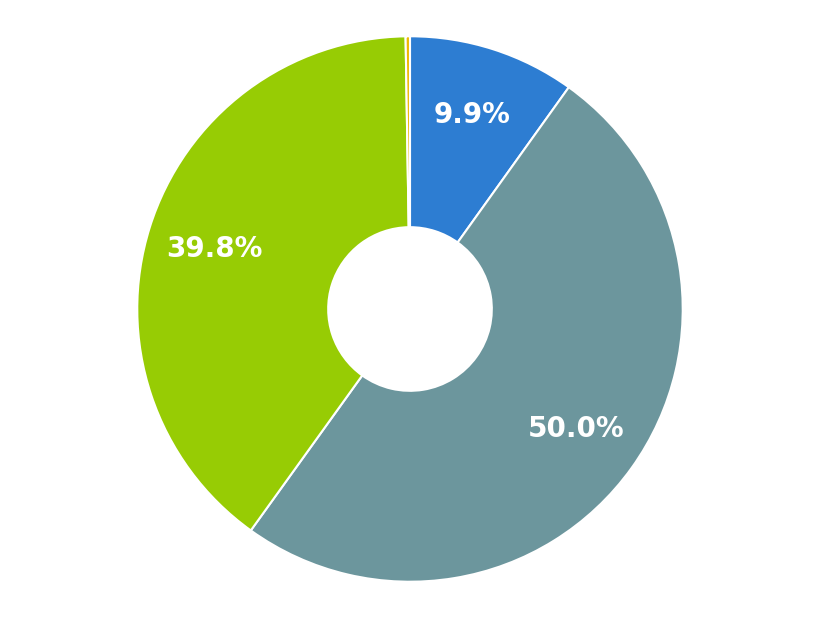
\includegraphics[width=0.75\textwidth]{\ThesisFigures/charts/topup-methods}
	\vspace{1em}  % add some space between chart and table

	% Then the table
	\small
	\begin{tabular}{@{}lrr@{}}
		\toprule
		\textbf{Payment Method}                & \textbf{Count} & \textbf{Total Value (CZK)} \\
		\midrule
		\colorindicator{chart2}Card terminal     & \fmtnum{8486}  & \fmtczk{7264503}           \\
		\colorindicator{chart3}Cash              & \fmtnum{7561}  & \fmtczk{5782570}           \\
		\colorindicator{chart1}Online pre top-up & \fmtnum{1634}  & \fmtczk{1436400}           \\
		\colorindicator{chart4}VIP issued        & \fmtnum{23}    & \fmtczk{37500}             \\
		\bottomrule
	\end{tabular}
	\caption{Top-Up Transactions by Payment Method}
	\label{fig:top-up-transactions-by-payment-method}
	\source
\end{figure}

Thanks to the results, it is clear how many funds did the system receive and by what means.

\begin{keytakeaways}
	\begin{itemize}
		\item Total top-up amount was~\bfmtczk{14520973}.
		\item Most used payment method was card terminal at the event with 50\% of all top-ups.
		\item Only around 10\% of the top-ups were done online.
	\end{itemize}
\end{keytakeaways}

%%% Cashflow / Sales Analysis
%%% --------------------------------------------------------------

\subsection{Sales Analysis}
\label{subsec:analysis-sales}
\begin{rqbox}
	\textit{\researchq{cashflow-total-sales}}
\end{rqbox}

The sales analysis was crucial for understanding the overall sales behavior and served as a basis for further insights tightly connected to the revenue sources.

To answer the research question, it was necessary to find all sales transactions and their respective sellers and to divide them into two groups: the direct organizer's sales and external vendors' sales.
And for better understanding, the sales were also grouped by the product categories (see~\autoref{tab:product-categories} for the list of categories).

The results show that the total sales of the event were~\bfmtczk{11711807} with the organizer's sales being~\bfmtczk{8240264} and the external vendors' sales~\bfmtczk{3471543}.

The organizer, most importantly, sold all the beer beverages and most of the non-alcoholic and alcoholic (spirits) beverages.
Whereas the external vendors sold mainly the food, wine beverages and other uncategorized products.
This can be seen in~\autoref{fig:sales-organizer-vs-vendors} below.

\begin{figure}[H]
	\centering
	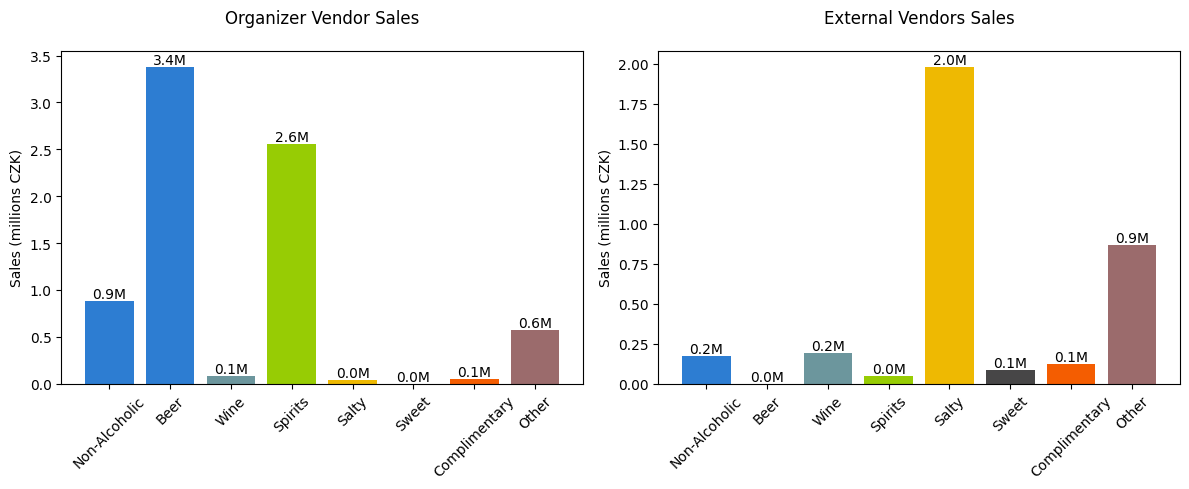
\includegraphics[width=0.99\textwidth]{\ThesisFigures/charts/sales-vendors}
	\caption{Sales of the Organizer vs. External Vendors}
	\label{fig:sales-organizer-vs-vendors}
	\source
\end{figure}

The organizer also sold not so little of uncategorized products, which after further investigation turned out to be ticket sales at the event amounting to~\bfmtczk{684700}.

In total, the organizer direct sales were \textbf{70\%} of the total sales, which is a significant portion, and thus the organizer itself has even bigger influence on the event's financial performance.

\begin{keytakeaways}
	\begin{itemize}
		\item Total sales of the event were~\bfmtczk{11711807}, where organizer sales were~\textbf{70\%} of the total.
		\item The organizer sold all beer beverages and the majority of the non-alcoholic and alcoholic beverages.
		\item The organizer also sold tickets at the event amounting to~\bfmtczk{684700}.
		\item External vendors sold mainly food, wine beverages, and other uncategorized products.
	\end{itemize}
\end{keytakeaways}

\todo{Better chart} % TODO

%%% Cashflow / Remaining Chip Balances
%%% --------------------------------------------------------------

\subsection{Remaining Chip Balances}
\label{subsec:analysis-remaining-balances}
\begin{rqbox}
	\textit{\researchq{cashflow-remaining-balance}}
\end{rqbox}

The remaining chip balances are crucial for the event organizer as they represent the potential revenue that can be still claimed.
Any unclaimed balances after a given refund period, which is usually up to 14~days after the event will be considered as organizer's taxable revenue.

Out of the total top-up amount of~\bfmtczk{14520973}, the total spent credit amounted to~\bfmtczk{10984945}, which left a total of~\bfmtczk{3536028} on the chips before refunds.
After refunds – done both at the event (\bfmtczk{15379}) and later via online bank refund requests (\bfmtczk{3163567}) – the remaining balance was reduced to~\bfmtczk{357082}.

However, this still included the artificially issued VIP credits with leftover balance of~\bfmtczk{12405}.
The system also reported integrity errors in the data, which resulted in a total of~\bfmtczk{10246} due to fraudulent activities performed by some attendees which were automatically suspended by the system.

This left the total unclaimed balance at~\bfmtczk{334431}, which has been claimed by the organizer as taxable revenue.

Since these numbers can be quite abstract, the results in a form of sankey diagram in~\autoref{fig:remaining-balances-sankey} below provide a clear picture of the flow of the funds.

\todo{Better chart} % TODO
\begin{figure}[H]
	\centering
	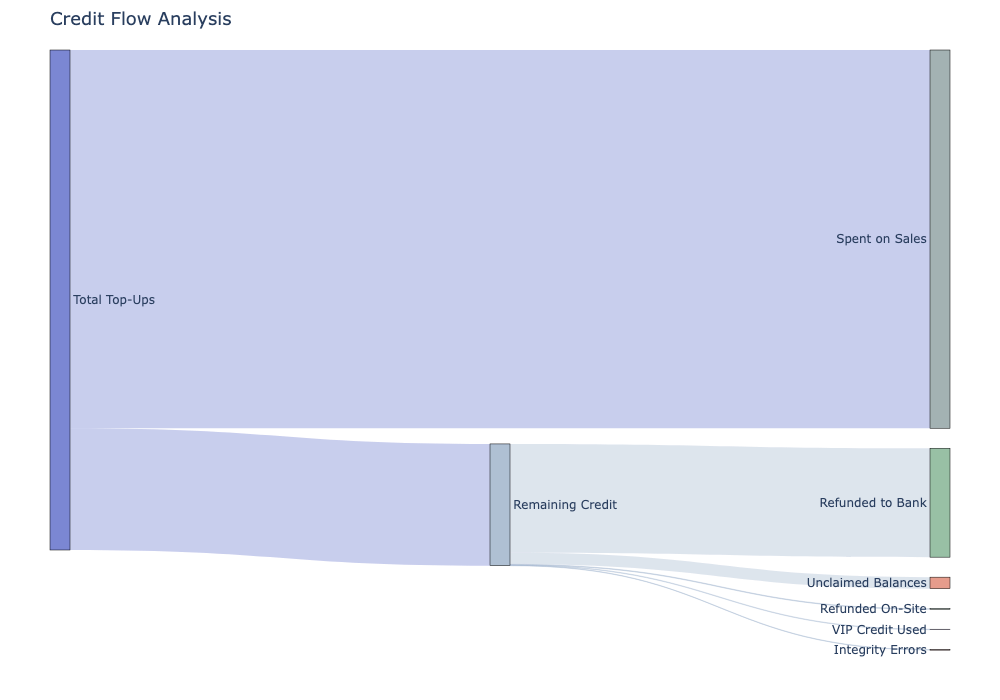
\includegraphics[width=0.99\textwidth]{\ThesisFigures/charts/balances-sankey}
	\caption{Remaining Chip Balances Sankey Diagram}
	\label{fig:remaining-balances-sankey}
	\source
\end{figure}

Thanks to this breakdown, it is clear how the remaining balances were reduced and what was the final outcome.
These results are important for the last part of this section, which is the total revenue of the organizer.

\begin{keytakeaways}
	\begin{itemize}
		\item Total unused credit was~\bfmtczk{3536028}.
		\item Credit refunded to customers was~\bfmtczk{3178946}.
		\item After VIP issued credits and system integrity error, the unclaimed balance was~\bfmtczk{334431}.
	\end{itemize}
\end{keytakeaways}

%%% Cashflow / Total Revenue of the Organizer
%%% --------------------------------------------------------------

\subsection{Total Revenue of the Organizer}
\label{subsec:analysis-total-revenue}
\begin{rqbox}
	\textit{\researchq{cashflow-total-revenue}}
\end{rqbox}

The festival's financial model is based on a combination of revenue streams.

The most important stream is the \textbf{commission from the vendor sales}, which is arranged in advance between the organizer and the vendors.
The commission is, in this case, a percentage (ranging from 15\% to 30\% depending on the deal) of the vendor sales amount without VAT\@.

Therefore, this required finding all sales transactions made at the external vendors' stands and calculating the commission based on the agreed percentage.
However, this was not a straightforward task, since a transaction could contain multiple products even from different vendors.

This required a more complex calculation, for which was used the previously mentioned data processing views which were designed for this purpose.
In the end, the total revenue from sales commissions was~\bfmtczkp[2]{820712,79}.

Another source of revenue is the \textbf{unclaimed chip balances}, which, after a credit refund period, are considered as taxable revenue for the organizer.
This, thanks to the previous subsection, was found to be~\bfmtczk{334431}.

\todo{Better chart} % TODO
\begin{figure}[H]
	\centering
	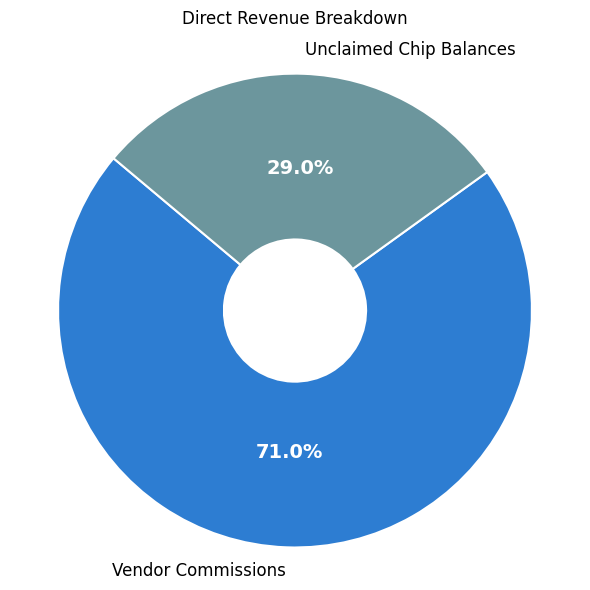
\includegraphics[width=0.48\textwidth]{\ThesisFigures/charts/revenue-sources-direct}
	\caption{Breakdown of Direct Revenue Streams}
	\label{fig:revenue-breakdown-direct}
	\source
\end{figure}

Currently totalling~\bfmtczkp[2]{1155143,79} is the direct revenue of the organizer from the event and can be seen in~\autoref{fig:revenue-breakdown-direct} above.

However, given the circumstances and setup of this event, there were also additional, but indirect revenue streams that were not included in the total revenue.
These include \textbf{the online ticket sales}, which were sold by the organizer and \textbf{the direct sales of the organizer}.
They were not included in the total direct revenue, as they may misinterpret the results since the analysis lacks expenses of the organizer.

If we were to include these, the total revenue would increase by~\bfmtczk{11179700} from the online ticket sales and~\bfmtczk{8240264} from the direct sales, which would result in a total revenue of~\bfmtczkp[2]{20575107,79}.

To better understand the revenue streams, the results are visualized in~\autoref{tab:revenue-summary-breakdown} and in~\autoref{fig:revenue-breakdown-total} below.

\begin{table}[H]
	\centering
	\begin{tabularx}{\textwidth}{|>{\columncolor{unicorn_blue!5}}X|>{\columncolor{unicorn_blue!5}}r|}
		\hline
		\rowcolor{unicorn_blue}
		\textbf{\color{white}Revenue Stream}         & \textbf{\color{white}Amount (CZK)} \\
		\hline
		\hline
		\colorindicator{chart1}Vendor Commissions      & \fmtczkp[2]{820712.79}             \\
		\colorindicator{chart2}Unclaimed Chip Balances & \fmtczk{334431}                    \\
		\hline
		\textbf{Total Direct Revenue}                  & \bfmtczkp[2]{1155143.79}           \\
		\hline
		\colorindicator{chart3}Online Ticket Sales     & \fmtczk{11179700}                  \\
		\colorindicator{chart4}Organizer Direct Sales  & \fmtczk{8240264}                   \\
		\hline
		\textbf{Total Revenue (All Streams)}           & \bfmtczkp[2]{20575107.79}          \\
		\hline
	\end{tabularx}
	\caption{Revenue Summary Breakdown}
	\label{tab:revenue-summary-breakdown}
\end{table}

\todo{Better chart} % TODO
\begin{figure}[H]
	\centering
	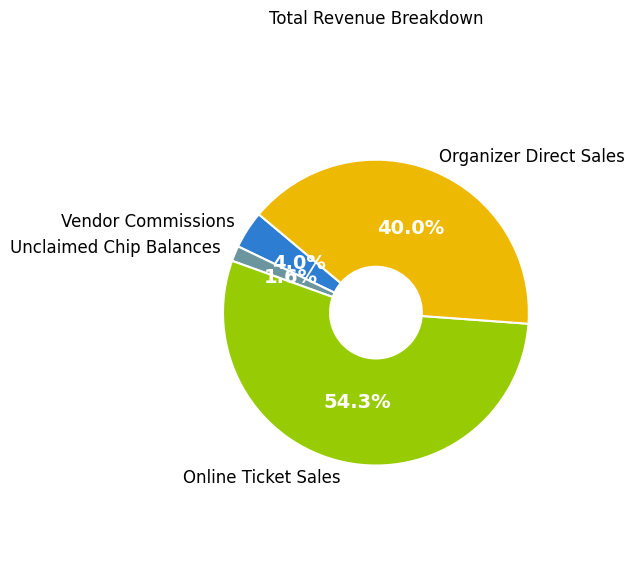
\includegraphics[width=0.75\textwidth]{\ThesisFigures/charts/revenue-sources-total}
	\caption{Breakdown of All Revenue Streams}
	\label{fig:revenue-breakdown-total}
	\source
\end{figure}

\begin{keytakeaways}
	\begin{itemize}
		\item Total direct revenue of the organizer was~\bfmtczkp[2]{1155143,79}.
		\item Vendor sale commission contributed to~approximately 71\% of the total direct revenue.
		\item With other indirect revenue streams, the total revenue would be~\bfmtczkp[2]{20575107,79}.
	\end{itemize}
\end{keytakeaways}

%%% Cashflow / Summary
%%% --------------------------------------------------------------

\subsection{Summary}
\label{subsec:analysis-cashflow-summary}

This section provided a comprehensive view of the festival's financial performance and cash flows.
The results covered the top-up transactions, sales analysis, remaining chip balances, and the total revenue of the organizer and contributed to a better understanding from the financial perspective of the festival.

Nevertheless, results covered in these subsections are only a part of the whole picture and can be interpreted in various ways.

For this particular challenge, a summarized cash flow diagram of payments was created, containing thus only the direct revenue streams.
This diagram can be seen in the~\autoref{fig:cash-flow-diagram} below.

\begin{figure}[H]
	\centering
	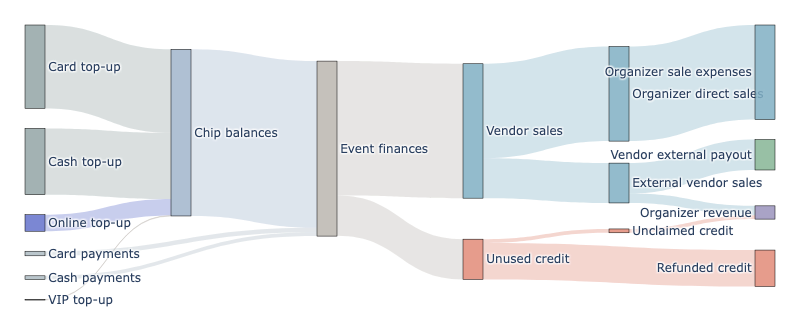
\includegraphics[width=0.99\textwidth]{\ThesisFigures/charts/revenue-cash-flows}
	\caption{Overall Cash Flow Diagram}
	\label{fig:cash-flow-diagram}
	\source
\end{figure}

This diagram provides a clear overview of the financial flows during the festival and nicely summarizes the results of this analysis.

\begin{keytakeaways}
	\begin{itemize}
		\item Total incoming money flow was~\bfmtczk{14520973} from top-up transactions and~\bfmtczk{726862} from non-chip sales.
		\item Total sales amounted to~\bfmtczk{11711807}.
		\item Which left a total of~\bfmtczk{3536028}~in unused credit before refunds.
		\item After refunds and non-refundable chips, the remaining balance left was~\bfmtczk{334431} claimed as taxable revenue.
		\item Commission from external vendor sales contributed to~\bfmtczkp[2]{820712,79}~of the total direct revenue.
		\item Together, the total direct revenue of the organizer was~\bfmtczkp[2]{1155143,79}.
	\end{itemize}
\end{keytakeaways}

%%% Section: Performance Indicators Analysis
%%% --------------------------------------------------------------


\section{Performance Indicators Analysis}
\label{sec:analysis-performance-indicators}

This section focuses on the performance indicators of the event.
The goal is to identify key metrics that can be used to further evaluate the event and its success.
The potential of this analysis is to measure the~\enquote{greatness}~and the size of the event in terms of performance.

This analysis sets out to answer other previously defined research questions related to the performance of the event.
Which, for purposes of this analysis, were slightly reordered and grouped into the two following subsections:
\begin{enumerate}
	\item \fullref{subsec:analysis-performance-indicators-transactions}
	\begin{itemize}
		\small
		\item \textit{\researchq{performance-transactions}}
		\item \textit{\researchq{performance-processing-during-peaks}}
		\item \textit{\researchq{performance-delays-downtimes}}
	\end{itemize}
	\item and~\fullref{subsec:analysis-performance-indicators-best}
	\begin{itemize}
		\small
		\item \textit{\researchq{performance-best-sale-points}}
		\item \textit{\researchq{performance-best-top-up-points}}
		\item \textit{\researchq{performance-best-vendors}}
		\item \textit{\researchq{performance-best-products}}
	\end{itemize}
\end{enumerate}

The results of this analysis should provide insights into the event's performance and help the organizer to understand the key metrics that can be used to evaluate the event's success.

%%% Performance / Transactions Processing Analysis
%%% --------------------------------------------------------------

\subsection{Transactions Processing Analysis}
\label{subsec:analysis-performance-indicators-transactions}

This subsection will focus on the processing of transactions during the event in pursuit of answering the three first research questions of this section.

\begin{rqbox}
	\textit{\researchq{performance-transactions}}
\end{rqbox}

This question actually consists of two sub-questions, which will be addressed separately.

The first part questions the total number of transactions processed during the event.
Which was actually pretty straightforward to answer, as the system was designed to track all transactions and their respective types.
The resulted total number of transactions was~\bfmtnum{141381} consisting of \bfmtnum{110854}~sales transactions, \bfmtnum{17726}~top-up transactions and~\bfmtnum{12801}~chip register transactions.

The second part focuses on rather time-related metrics and asks about the processing peak times during the festival.
For this part, it was necessary to spread out the above transactions over the time and find the peaks.

The results in~\autoref{fig:transactions-processing-peaks} below show the distribution of the processed transactions over time.
It clearly identifies the peak on the last day of the festival at 18:00 amounting to~\bfmtnum{8986}~transactions.

\todo{Better chart} % TODO
\begin{figure}[H]
	\centering
	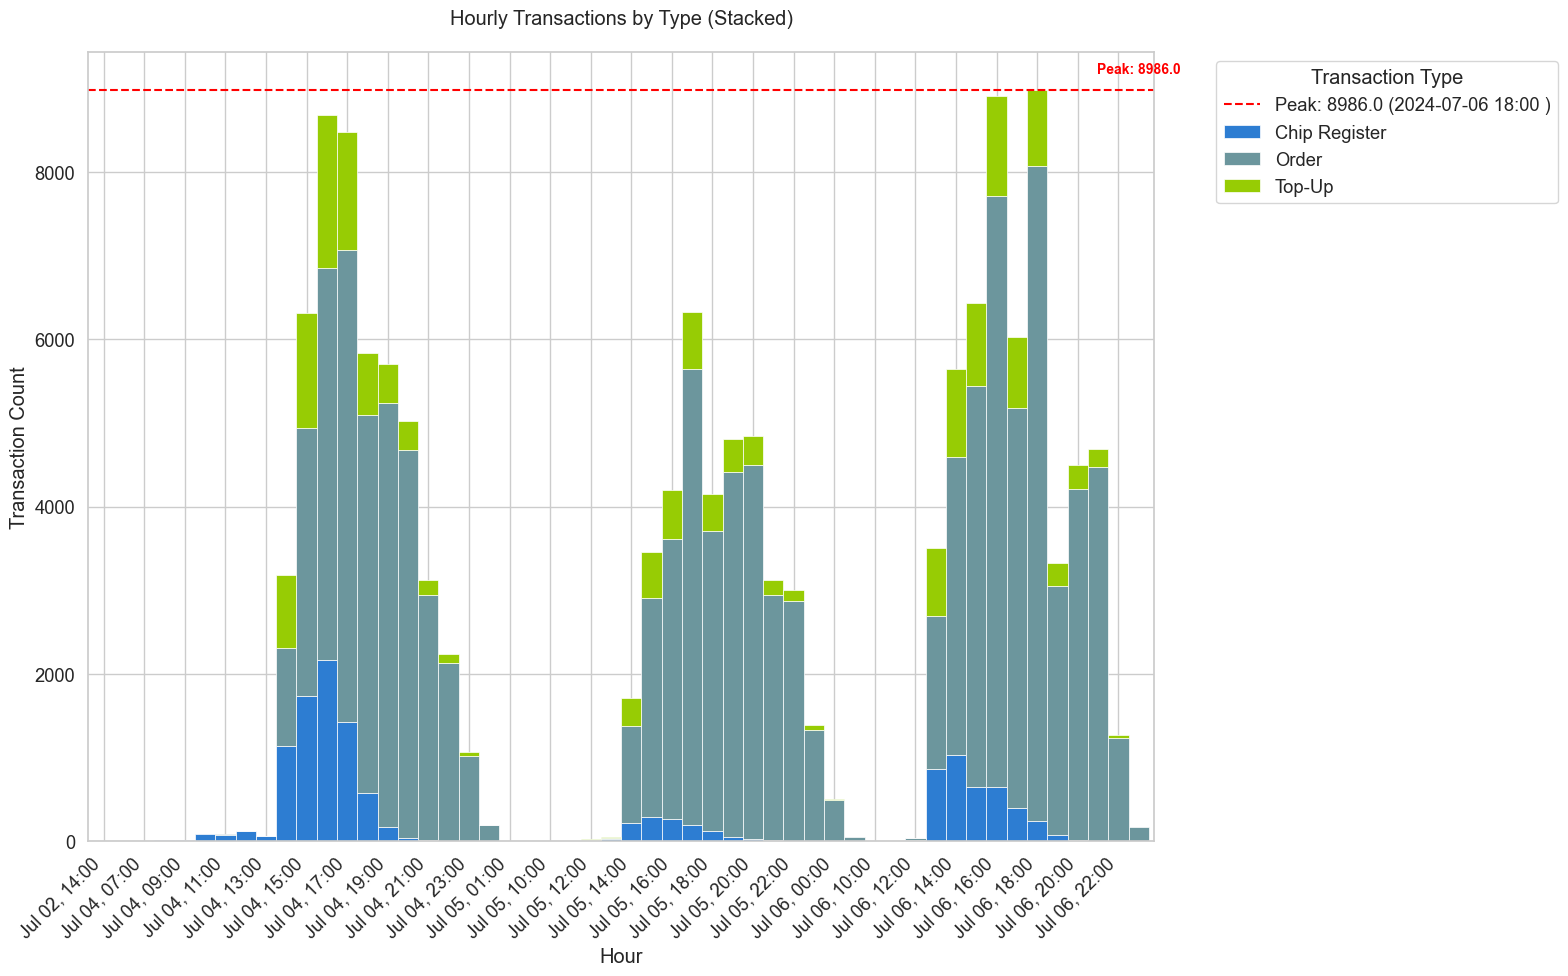
\includegraphics[width=0.99\textwidth]{\ThesisFigures/charts/performance-transactions-in-time}
	\caption{Transactions Processing Peaks}
	\label{fig:transactions-processing-peaks}
	\source
\end{figure}

\begin{keytakeaways}
	\begin{itemize}
		\item Total number of transactions processed was~\bfmtnum{141381} consisting mainly (7̃8\%) of order transactions.
		\item The peak of transactions was on the last day of the festival at 18:00 with~\bfmtnum{8986}~transactions processed at that hour.
	\end{itemize}
\end{keytakeaways}

The following two questions (\autoref{rq:performance-processing-during-peaks}~and~\autoref{rq:performance-delays-downtimes}), focus on processing times and potential delays during the event.

\begin{rqbox}
	\textit{\researchq{performance-processing-during-peaks}}
\end{rqbox}

The answer to this question is closely related to the previous one, as it requires the identification of the processing times during the peak times, which were already identified.

It required finding the average processing time, meaning difference between the transaction creation and its completion times.

\begin{info-box}{What causes the processing time?}
	\textit{
		Time when the transaction is created is the time when the in-place offline-supported system created the transaction, and the processed time is later when the central system receives the transaction and processes it.
		The delays can be caused by various factors, such as network latency, offline mode active, system load, or even the transaction type.
	}
\end{info-box}

The results show that the average processing time during the peak times was approximately~\bfmtnum{40}~seconds.

When slightly changing the displayed data, we also get the answer to the~\autoref{rq:performance-delays-downtimes} about the potential delays and downtimes during the event.

\begin{rqbox}
	\textit{\researchq{performance-delays-downtimes}}
\end{rqbox}

The chart in the~\autoref{fig:rq7-delays-in-processing}~shows the distribution of the processing times over the time and identifies one high processing peak of approximately~\bfmtnum{13}~minutes.
This is highly unusual and indicates a vendor misuse of the system or accidentally put the system into offline mode.

\todo{Better chart} % TODO
\begin{figure}[H]
	\centering
	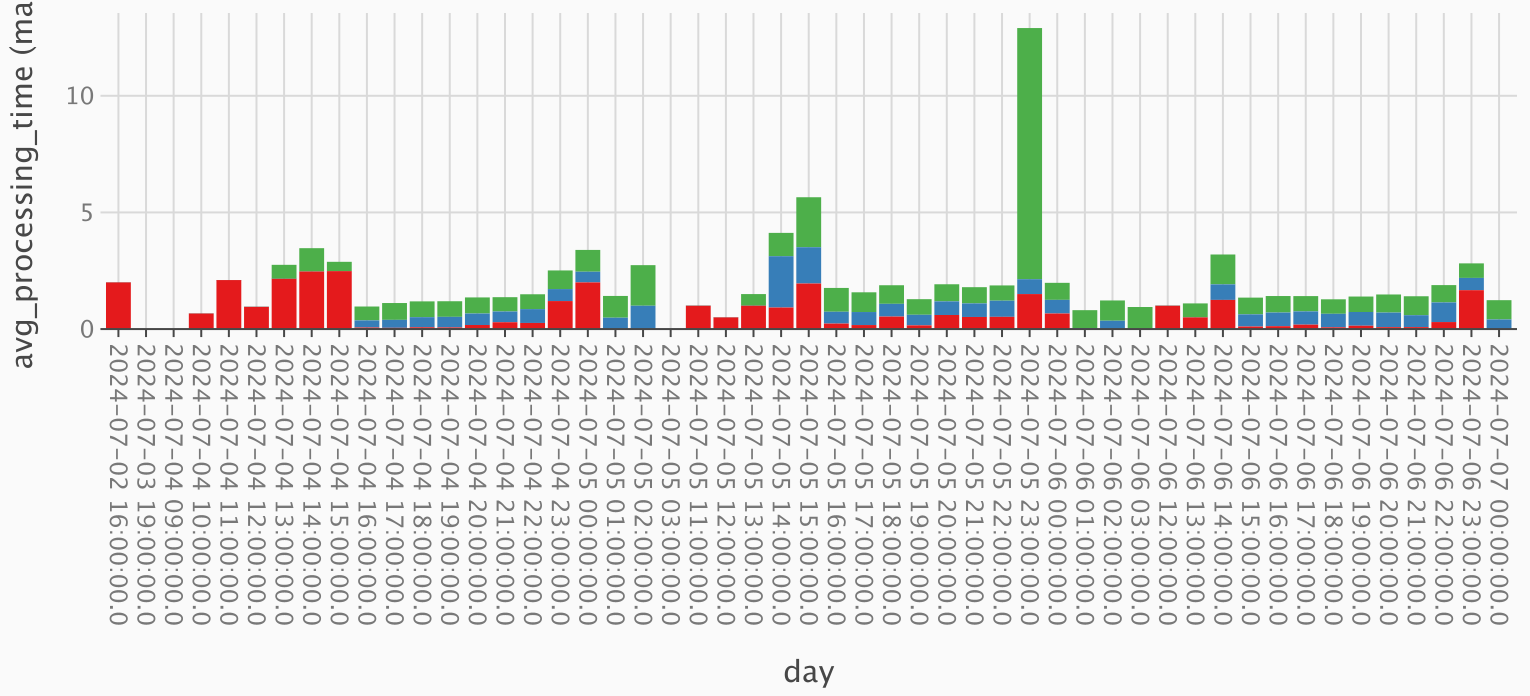
\includegraphics[width=0.99\textwidth]{\ResultsDir/rq7-delays-in-processing}
	\caption{Transaction Processing Peaks}
	\label{fig:rq7-delays-in-processing}
	\source
\end{figure}

Other high peaks are visible on the second day in the afternoon with ~ \bfmtnum{5}~minutes processing time, which was probably caused by the initial load on that day.

\begin{keytakeaways}
	\begin{itemize}
		\item The average processing time during the peak times was~\bfmtnum{40}~seconds.
		\item The highest processing peak was approximately~\bfmtnum{13}~minutes, indicating a potential misuse of the system.
		\item Other high peaks were visible on the second day in the afternoon with ~ \bfmtnum{5}~minutes processing time.
	\end{itemize}
\end{keytakeaways}

These results provide insights into the system's performance during the event, its reliability, and potential bottlenecks.
It also shows the festival's popularity and the system's ability to handle the load.

%%% Performance / Best Sale & Top-Up Points, Vendors, and Products Analysis
%%% --------------------------------------------------------------

\subsection{Best Sale \& Top-Up Points, Vendors, and Products Analysis}
\label{subsec:analysis-performance-indicators-best}
In this subsection, the main goal will be to address the last four research questions of this section and provide insights into the best: selling points, top-up points, vendors, and products.

The problem with these question statements is that they are quite broad and can be interpreted in various ways.
What does a~\enquote{best} mean in this context?

It can be the most profitable, the best rated, the most visited, etc.
But since we are exploring the performance indicators, the best should be understood as the~\enquote{busiest}.
Which in terms of the system and this analysis should mean \textbf{the most transactions created} and the point's ability to handle the load.

%%% Performance / Best Sale & Top-Up Points, Vendors, and Products Analysis / Best Sale Points
%%% --------------------------------------------------------------

\subsubsection{Best Top-Up Points}
\label{subsubsec:analysis-best-top-up-points}
The first focus will be on the best top-up points since unlike the selling points, vendors and products, the top-up points are not linked to any specific product or vendor.
\begin{rqbox}
	\textit{\researchq{performance-best-top-up-points}}
\end{rqbox}

To find these results, it required finding all top-up transactions, aggregate them in a bucket-like time frame and finally calculate their total counts, max peaks and averages over time.

This resulted in the following findings in the~\autoref{tab:best-topup-points} below.

\begin{table}[htbp]
	\centering
	\small
	\begin{tabularx}{\textwidth}{
		|>{\columncolor{unicorn_blue!5}\centering\arraybackslash}p{1cm}
		|>{\columncolor{unicorn_blue!5}\raggedright\arraybackslash}X
		|>{\columncolor{unicorn_blue!5}\raggedleft\arraybackslash}p{2.5cm}
		|>{\columncolor{unicorn_blue!5}\raggedleft\arraybackslash}p{2.5cm}
		|>{\columncolor{unicorn_blue!5}\raggedleft\arraybackslash}p{2.5cm}|}
		\hline
		\rowcolor{unicorn_blue}
		\textbf{}
		& \textbf{\color{white}Top-Up point}
		& \textbf{\color{white}Customers}
		& \textbf{\color{white}Transactions}
		& \textbf{\color{white}Max trx./h}
		\\\hline\hline
		% first rows
		\csvreader[
		head to column names,
		late after line={\\\hline},
		filter={\thecsvinputline<6}
		]{\ResultsDir/rq9-best-topup-points.csv}{
			entity=\colentity,
			customer_count=\colcustomers,
			transaction_count=\coltrxcount,
			max_hourly_peak=\colhourlypeak
		}{
			\the\numexpr\thecsvinputline-1
			& \colentity
			& \num[group-separator={,}]{\colcustomers}
			& \num[group-separator={,}]{\coltrxcount}
			& \num[group-separator={,}]{\colhourlypeak}
		}
		% separator
		\noalign{\vspace{1mm}}
		\multicolumn{5}{c}{\footnotesize{\textellipsis}}
		\\
		\noalign{\vspace{1mm}}
		\hline
		% middle rows
		\csvreader[
		head to column names,
		late after line={\\\hline},
		filter={\thecsvinputline>15 \AND \thecsvinputline<20}
		]{\ResultsDir/rq9-best-topup-points.csv}{
			entity=\colentity,
			customer_count=\colcustomers,
			transaction_count=\coltrxcount,
			max_hourly_peak=\colhourlypeak
		}{
			\the\numexpr\thecsvinputline-1
			& \colentity
			& \num[group-separator={,}]{\colcustomers}
			& \num[group-separator={,}]{\coltrxcount}
			& \num[group-separator={,}]{\colhourlypeak}
		}
		% separator
		\noalign{\vspace{1mm}}
		\multicolumn{5}{c}{\footnotesize{\textellipsis}}
		\\
		\noalign{\vspace{1mm}}
		\hline
		% last rows
		\csvreader[
		head to column names,
		late after line={\\\hline},
		filter={\thecsvinputline>25}
		]{\ResultsDir/rq9-best-topup-points.csv}{
			entity=\colentity,
			customer_count=\colcustomers,
			transaction_count=\coltrxcount,
			max_hourly_peak=\colhourlypeak
		}{
			\the\numexpr\thecsvinputline-1
			& \colentity
			& \num[group-separator={,}]{\colcustomers}
			& \num[group-separator={,}]{\coltrxcount}
			& \num[group-separator={,}]{\colhourlypeak}
		}
	\end{tabularx}
	\caption{Best Top-Up Points}
	\label{tab:best-topup-points}
\end{table}

This indicates that the most busy top-up points were somehow evenly distributed with approximately around \textbf{1000~transactions} processed during the event with average peaks of around \textbf{100~transactions/hour}.
The least busy top-up points were the specific ones, such as the Support tent, VIP and Accreditation points, which were not used so much for top-ups.

The overall distribution, shown in the~\autoref{fig:best-topup-points}, also shows that Top-up points were more busy than Check-in points.
That makes sense because the top-ups were done more frequently than the initial check-ins, but the check-ins were done in a more concentrated time frame.

\begin{figure}[H]
	\centering
	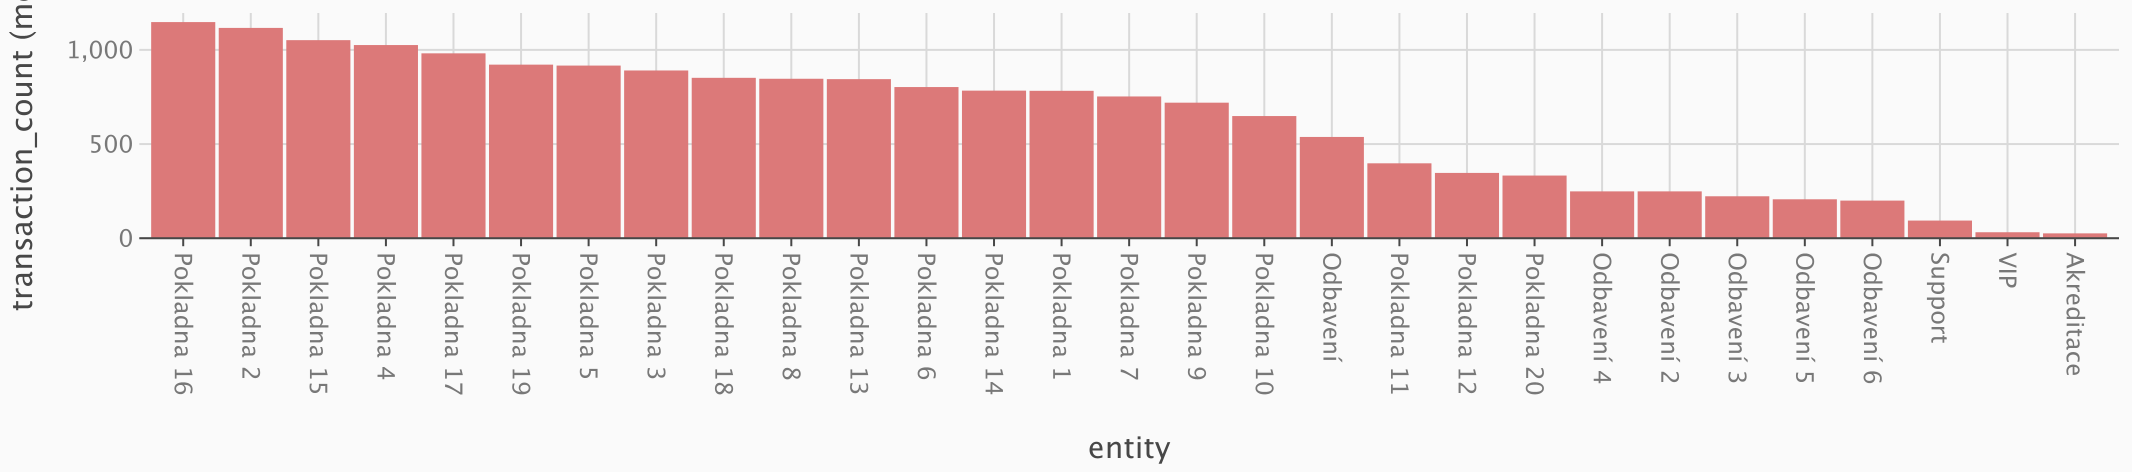
\includegraphics[width=0.99\textwidth]{\ResultsDir/rq9-best-topup-points}
	\caption{Best Top-Up Points}
	\label{fig:best-topup-points}
	\source
\end{figure}
\todo{Better chart} % TODO

Especially \textbf{Odbavení} point processed only~\bfmtnum{529}~transactions but peaked at~\bfmtnum{125}~transactions per hour, which was much higher than the other check-in points and even higher than the best top-up points.

\begin{keytakeaways}
	\begin{itemize}
		\item The most busy top-up points processed around~\bfmtnum{1000}~transactions during the event.
		\item The average peak of the top-up points was around~\bfmtnum{100}~transactions per hour.
		\item The least busy top-up points were the specific ones, such as the Support tent, VIP and Accreditation points.
		\item Check-in points were less busy than the top-up points, but the \textbf{Odbavení} point peaked at~\bfmtnum{125}~transactions per hour.
	\end{itemize}
\end{keytakeaways}

%%% Performance / Best Sale & Top-Up Points, Vendors, and Products Analysis / Best Sale Points
%%% --------------------------------------------------------------

\subsubsection{Best Sale Points}
\label{subsubsec:analysis-best-sale-points}

The next focus will be on the best sale points, which are the points where the most orders were created.

\begin{rqbox}
	\textit{\researchq{performance-best-sale-points}}
\end{rqbox}

The process of finding the best sale points was similar to the previous one, but this time it required finding all sales transactions and their respective points.

Out of total of~\bfmtnum{145}~sale points, the best place was undeniable the \textbf{L20 PIVNÍ STAN 1} with total~\bfmtnum{10114}~orders processed and the maximum peak of~\bfmtnum{840}~orders per hour.

Another interesting fact is the total unique users processed at the places.
Where again the \textbf{L20 PIVNÍ STAN 1} processed~\bfmtnum{9159}~unique customers which, out of \bfmtnum{10009}~active customers, is a significant portion (\bfmtnump[2]{91.50}{}\%) of the total.

\begin{table}[htbp]
	\centering
	\small
	\begin{tabularx}{\textwidth}{
		|>{\columncolor{unicorn_blue!5}\centering\arraybackslash}p{1cm}
		|>{\columncolor{unicorn_blue!5}\raggedright\arraybackslash}X
		|>{\columncolor{unicorn_blue!5}\raggedleft\arraybackslash}p{2.5cm}
		|>{\columncolor{unicorn_blue!5}\raggedleft\arraybackslash}p{2.5cm}
		|>{\columncolor{unicorn_blue!5}\raggedleft\arraybackslash}p{2.5cm}|}
		\hline
		\rowcolor{unicorn_blue}
		\textbf{}
		& \textbf{\color{white}Sale Point}
		& \textbf{\color{white}Customers}
		& \textbf{\color{white}Orders}
		& \textbf{\color{white}Max orders./h}
		\\\hline\hline
		% first rows
		\csvreader[
		head to column names,
		late after line={\\\hline},
		filter={\thecsvinputline<9}
		]{\ResultsDir/rq8-best-sale-points.csv}{
			entity=\colentity,
			customer_count=\colcustomers,
			transaction_count=\coltrxcount,
			max_hourly_peak=\colhourlypeak
		}{
			\the\numexpr\thecsvinputline-1
			& \colentity
			& \num[group-separator={,}]{\colcustomers}
			& \num[group-separator={,}]{\coltrxcount}
			& \num[group-separator={,}]{\colhourlypeak}
		}
		% separator
		\noalign{\vspace{1mm}}
		\multicolumn{5}{c}{\footnotesize{\textellipsis}}
		\\
		\noalign{\vspace{1mm}}
		\hline
		% last rows
		\csvreader[
		head to column names,
		late after line={\\\hline},
		filter={\thecsvinputline>132}
		]{\ResultsDir/rq8-best-sale-points.csv}{
			entity=\colentity,
			customer_count=\colcustomers,
			transaction_count=\coltrxcount,
			max_hourly_peak=\colhourlypeak
		}{
			\the\numexpr\thecsvinputline-1
			& \colentity
			& \num[group-separator={,}]{\colcustomers}
			& \num[group-separator={,}]{\coltrxcount}
			& \num[group-separator={,}]{\colhourlypeak}
		}
	\end{tabularx}
	\caption{Best Sale Points}
	\label{tab:best-sale-points}
\end{table}

Based on this particular finding, we can assume that in the following analysis - the best vendors and products - the product preferences will be highly in favor of the beer beverages.
And thus the best vendor will probably be the organizer, as they sold all the beer beverages at the festival.

\begin{keytakeaways}
	\begin{itemize}
		\item The best sale point was the \textbf{L20 PIVNÍ STAN 1} with total~\bfmtnum{10114}~orders processed, which was~\bfmtnump[2]{9.12}\% of the total orders created.
		\item The best sale point peaked at~\bfmtnum{840}~orders per hour.
		\item The \textbf{L20 PIVNÍ STAN 1} processed~\bfmtnum{9159}~unique customers, which was~\bfmtnump[2]{91.50}\% of all active customers.
	\end{itemize}
\end{keytakeaways}

In conclusion to these two questions, the results show clearly the busiest points of the festival and their ability to handle the load.
However, the results can be visualized in a more interactive way, which would provide a better understanding of the data.

One especially interesting visualization of the best sale and top-up points would be a heatmap of the festival area with the points and their respective transaction counts.
As this was initially intended to be part of the analysis, it was unfortunately not possible to create it due to the lack of the necessary data.

%%% Performance / Best Sale & Top-Up Points, Vendors, and Products Analysis / Best Vendors
%%% --------------------------------------------------------------

\subsubsection{Best Vendors}
\label{subsubsec:analysis-best-vendors}

To analyze the best vendors, in terms of performance, the same approach as with the sale points will be used.
\begin{rqbox}
	\textit{\researchq{performance-best-vendors}}
\end{rqbox}

The results in the~\autoref{tab:best-vendors} below show the distribution of the processed orders over the vendors.

\begin{table}[htbp]
	\centering
	\small
	\begin{tabularx}{\textwidth}{
		|>{\columncolor{unicorn_blue!5}\centering\arraybackslash}p{1cm}
		|>{\columncolor{unicorn_blue!5}\raggedright\arraybackslash}X
		|>{\columncolor{unicorn_blue!5}\raggedleft\arraybackslash}p{2.5cm}
		|>{\columncolor{unicorn_blue!5}\raggedleft\arraybackslash}p{2.5cm}|}
		\hline
		\rowcolor{unicorn_blue}
		\textbf{}
		& \textbf{\color{white}Vendor}
		& \textbf{\color{white}Customers}
		& \textbf{\color{white}Orders}
		\\\hline\hline
		% first rows
		\csvreader[
		head to column names,
		late after line={\\\hline},
		filter={\thecsvinputline<9}
		]{\ResultsDir/rq10-best-vendors.csv}{
			legal_name=\colentity,
			customer_count=\colcustomers,
			transaction_count=\coltrxcount,
		}{
			\the\numexpr\thecsvinputline-1
			& \colentity
			& \num[group-separator={,}]{\colcustomers}
			& \num[group-separator={,}]{\coltrxcount}
		}
		% separator
		\noalign{\vspace{1mm}}
		\multicolumn{5}{c}{\footnotesize{\textellipsis}}
		\\
		\noalign{\vspace{1mm}}
		\hline
		% last rows
		\csvreader[
		head to column names,
		late after line={\\\hline},
		filter={\thecsvinputline>25}
		]{\ResultsDir/rq10-best-vendors.csv}{
			legal_name=\colentity,
			customer_count=\colcustomers,
			transaction_count=\coltrxcount,
		}{
			\the\numexpr\thecsvinputline-1
			& \colentity
			& \num[group-separator={,}]{\colcustomers}
			& \num[group-separator={,}]{\coltrxcount}
		}
	\end{tabularx}
	\caption{Best Vendors}
	\label{tab:best-vendors}
\end{table}

As predicted in the previous section, the best vendor was the organizer, which processed the most orders and customers.
The total of~\bfmtnum{89217}~orders was processed by the organizer, which was~\bfmtnump[2]{80.04}\% of the total orders created and served~\bfmtnum{9831}~unique customers, which was~\bfmtnump[2]{98.22}\% of all active customers.

The second-best vendor, out of~\bfmtnum{27}~total, was some \textbf{Seller 05} with about~\bfmtnum{84104} orders less than the organizer.

In these results, we did not go after the hourly maximums, as in the previous questions, as the vendors were not time-bound and could have been at multiple places simultaneously.
The results would not be so relevant and would not provide any additional insights.

\begin{keytakeaways}
	\begin{itemize}
		\item The best vendor was the organizer, which processed~\bfmtnum{89217}~orders (\bfmtnump[2]{80.04}\%~of the total orders).
		\item The best vendor served~\bfmtnum{9831}~unique customers (\bfmtnump[2]{98.22}\%~of all active customers).
		\item The second-best vendor was behind around~\bfmtnum{84104}~orders less than the best vendor.
	\end{itemize}
\end{keytakeaways}

%%% Performance / Best Sale & Top-Up Points, Vendors, and Products Analysis / Best Products
%%% --------------------------------------------------------------

\subsubsection{Best Products}
\label{subsubsec:analysis-best-products}

The last focus will be on the best products, which are the products that were sold the most during the event.

\begin{rqbox}
	\textit{\researchq{performance-best-products}}
\end{rqbox}

Previously, the best products were predicted to be the beer beverages, as the organizer sold all the beer beverages at the festival.

The results in the~\autoref{tab:best-products} below somehow confirm this prediction as the very best product was a returnable cup – \textbf{Kelímek – záloha} and the next four best products were beer beverages:

\begin{table}[htbp]
	\centering
	\small
	\begin{tabularx}{\textwidth}{
		|>{\columncolor{unicorn_blue!5}\centering\arraybackslash}p{1cm}
		|>{\columncolor{unicorn_blue!5}\raggedright\arraybackslash}X
		|>{\columncolor{unicorn_blue!5}\raggedleft\arraybackslash}p{2.5cm}
		|>{\columncolor{unicorn_blue!5}\raggedleft\arraybackslash}p{2.5cm}
		|>{\columncolor{unicorn_blue!5}\raggedleft\arraybackslash}p{2.5cm}|}
		\hline
		\rowcolor{unicorn_blue}
		\textbf{}
		& \textbf{\color{white}Product}
		& \textbf{\color{white}Sales}
		& \textbf{\color{white}Refunds}
		& \textbf{\color{white}Customers}
		\\\hline\hline
		% first rows
		\csvreader[
		head to column names,
		late after line={\\\hline},
		filter={\thecsvinputline<9}
		]{\ResultsDir/rq11-best-products.csv}{
			product_name=\colproduct,
			customer_count=\colcustomers,
			sales_count=\colsalescount,
			refund_count=\colrefundcount
		}{
			\the\numexpr\thecsvinputline-1
			& \colproduct
			& \num[group-separator={,}]{\colsalescount}
			& \num[group-separator={,}]{\colrefundcount}
			& \num[group-separator={,}]{\colcustomers}
		}
		% separator
		\noalign{\vspace{1mm}}
		\multicolumn{5}{c}{\footnotesize{\textellipsis}}
		\\
		\noalign{\vspace{1mm}}
		\hline
		% last rows
		\csvreader[
		head to column names,
		late after line={\\\hline},
		filter={\thecsvinputline>326}
		]{\ResultsDir/rq11-best-products.csv}{
			product_name=\colproduct,
			customer_count=\colcustomers,
			sales_count=\colsalescount,
			refund_count=\colrefundcount
		}{
			\the\numexpr\thecsvinputline-1
			& \colproduct
			& \num[group-separator={,}]{\colsalescount}
			& \num[group-separator={,}]{\colrefundcount}
			& \num[group-separator={,}]{\colcustomers}
		}
	\end{tabularx}
	\caption{Best Products}
	\label{tab:best-products}
\end{table}

As there were more than \bfmtnum{300}~products sold during the event, a better visualization of the results would be a bar chart showing the best product categories instead of individual products.
This can be seen in the~\autoref{fig:best-product-category} below.

\begin{figure}[H]
	\centering
	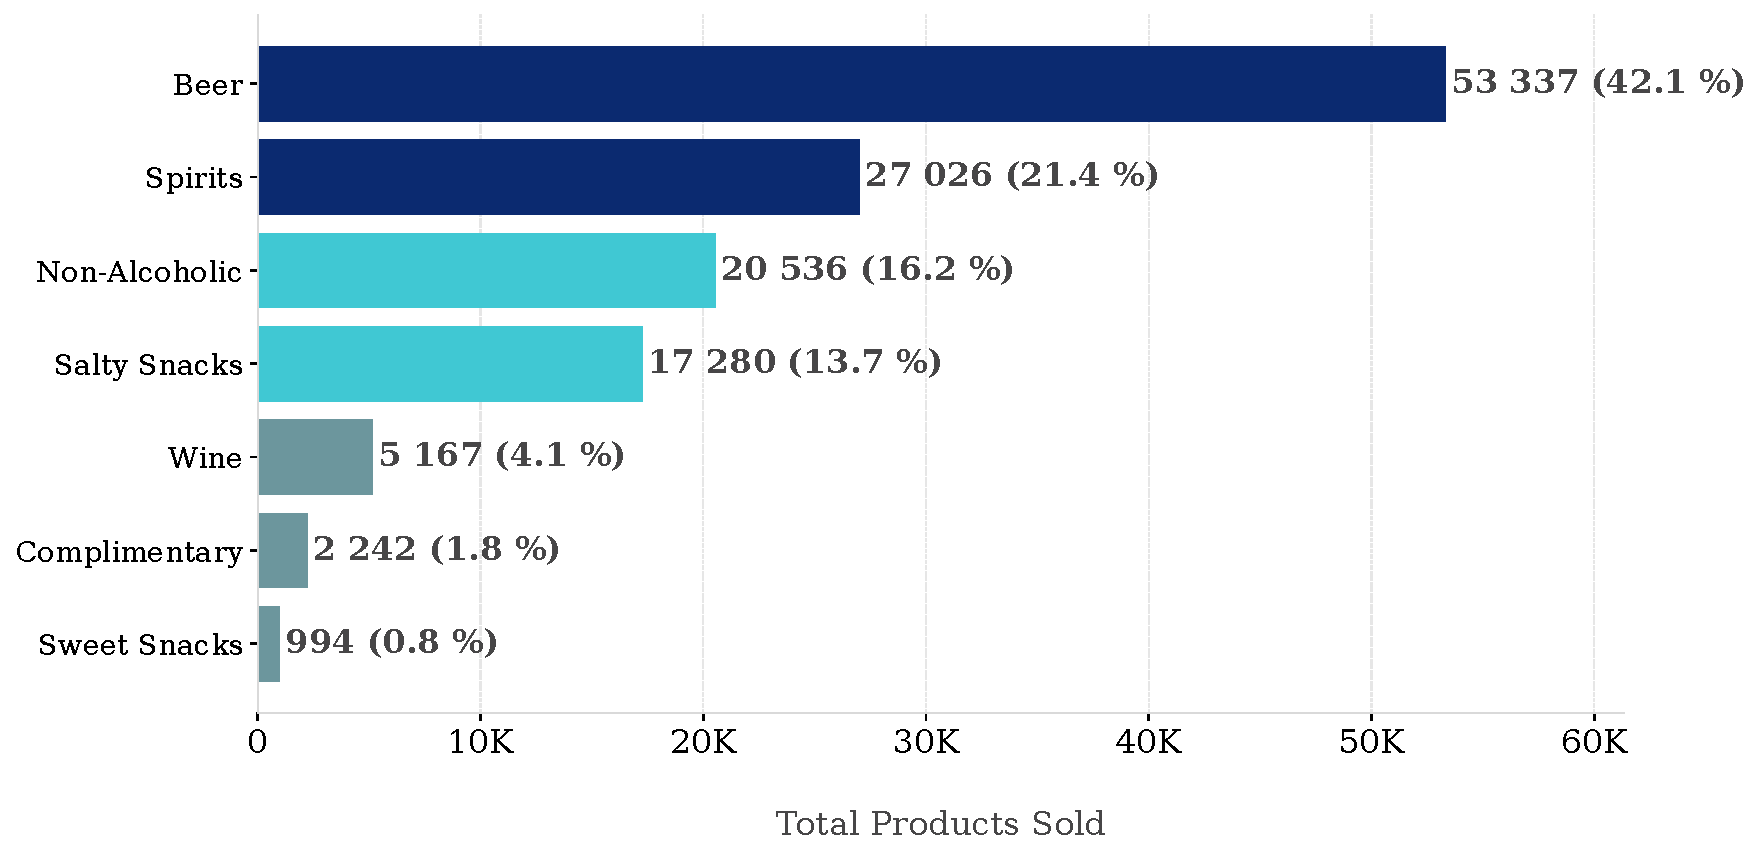
\includegraphics[width=0.99\textwidth]{\ResultsDir/rq11-best-product-category}
	\caption{Best Products by Category}
	\label{fig:best-product-category}
	\source
\end{figure}
\todo{Better chart} % TODO

This chart now confirms the prediction about the beer beverages, as the \textbf{Beer} (Pivo) category was the most sold during the event with a little more than~\bfmtnum{40000}~orders processed.

\begin{keytakeaways}
	\begin{itemize}
		\item The best product was a returnable cup followed by beer beverages.
		\item Prediction about the beer beverages was confirmed, as the \textbf{Beer} (Pivo) category was the most sold during the event.
	\end{itemize}
\end{keytakeaways}

This last analysis provided insights into the best products, which confirmed the previous predictions and will now serve as a basis for the next section, where the beverage consumption will be analyzed.

%%% Performance / Summary
%%% --------------------------------------------------------------

\subsection{Summary}
\label{subsec:analysis-performance-indicators-summary}

Thanks to this section, the performance indicators of the event were analyzed, and the key metrics were identified.
The results analyzed the transactional processing performance, identified several peak points during the event, and provided insights into the best sale points, top-up points, vendors, and products.
Providing a better understanding of the event's performance and giving more context for the next analysis dealing with the beverage consumption.

%%% Section: Beverage Consumption Analysis
%%% --------------------------------------------------------------


\section{Beverage Consumption Analysis}
\label{sec:analysis-beverage-consumption}

This section will provide a detailed analysis of beverage consumption, which was previously established as the most significant aspect of the event.

It should offer insights into overall consumption, detailed information on returnable cups, the most often drank beverages, and the leading beverage brands, addressing the previously established inquiries.

This section will address the next six research questions, after a minor logical reorganization into three groups:
\begin{enumerate}
	\item \fullref{subsec:analysis-beverage-returnable-cups}
	\begin{itemize}
		\small
		\item \textit{\researchq{beverage-returnable-cups}}
	\end{itemize}
	\item \fullref{subsec:analysis-beverage-total-consumption}
	\begin{itemize}
		\small
		\item \textit{\researchq{beverage-total-consumption}}
		\item \textit{\researchq{beverage-popular-category}}
	\end{itemize}
	\item and~\fullref{subsec:analysis-beverage-popular-brands}.
	\begin{itemize}
		\small
		\item \textit{\researchq{beverage-top-beer}}
		\item \textit{\researchq{beverage-top-non-alcoholic}}
		\item \textit{\researchq{beverage-top-alcoholic}}
	\end{itemize}
\end{enumerate}

%%% Beverage / Returnable Cups Analysis
%%% --------------------------------------------------------------

\subsection{Returnable Cups Analysis}
\label{subsec:analysis-beverage-returnable-cups}

Due to the little alteration of the local database and the previously referenced data in~\autoref{subsec:data-methodology-local-database-modifications}, it became possible to monitor the returnable cups and their associated transactions.

This capability, previously absent, should enhance comprehension of product sales and the utilization of returnable cups.

\begin{rqbox}
	\textit{\researchq{beverage-returnable-cups}}
\end{rqbox}

To figure out the results, it was essential to analyze the actual contents of the transactions rather than merely identifying transactions including returnable cups,
as a single transaction may encompass many products and hence multiple returnable cups.
The organizer sold the cups for a price of ~\fmtczk{70} with a ~\fmtnum{21}\% VAT.\

Upon calculating the total number of issued and returned cups, the results depicted in~\autoref{fig:returnable-cups}~below illustrate the distribution of returnable cups throughout the event.

\begin{figure}[H]
	\centering
	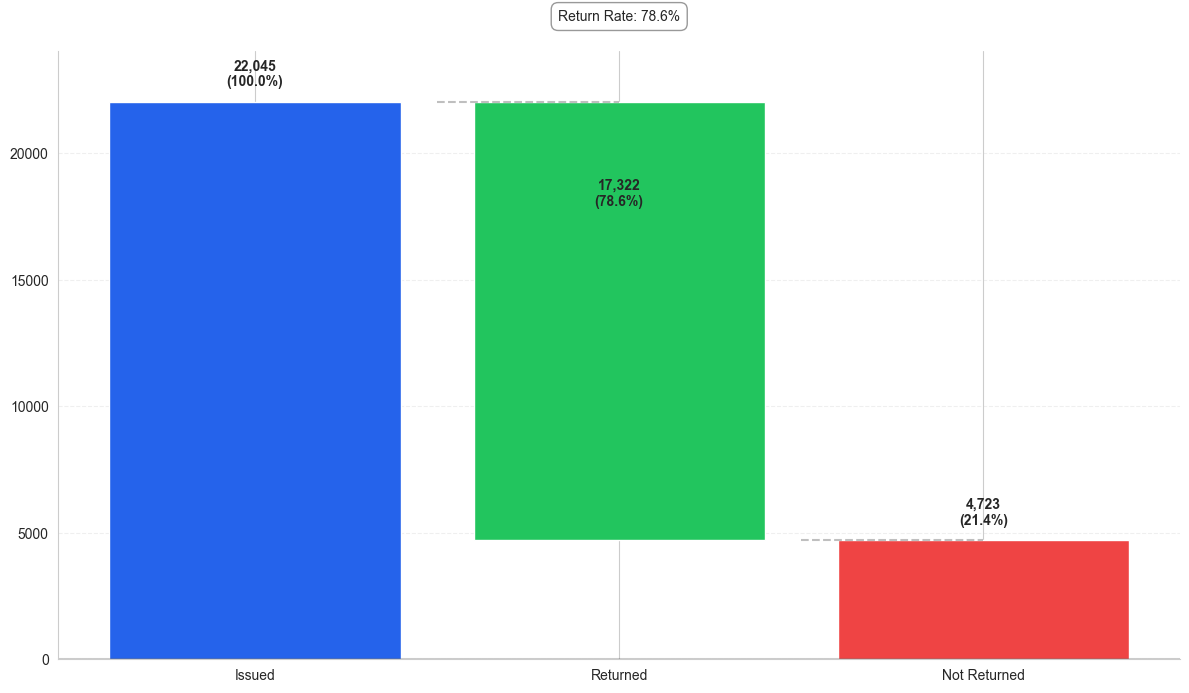
\includegraphics[width=0.99\textwidth]{\ResultsDir/rq13-returnable-cups}
	\caption{Returnable Cups}
	\label{fig:returnable-cups}
	\source
\end{figure}

The data indicate that a total of~\bfmtnum{20045}~cups was distributed during the event, with only~\bfmtnum{17322}~cups returned, yielding a return rate of~\bfmtnump[2]{78.60}\%.

This, however, does not imply that the remaining~\bfmtnum{4723}~cups were lost or regarded as a loss, as the cups were purchased.
Most unreturned cups can be presumed to have been retained as souvenirs.

\begin{keytakeaways}
	\begin{itemize}
		\item The total of~\bfmtnum{20045}~cups were issued during the festival.
		\item Only~\bfmtnum{17322}~cups returned resulted in a~\bfmtnump[2]{78.60}\%~return rate.
	\end{itemize}
\end{keytakeaways}

%%% Beverage / Total Consumption Analysis
%%% --------------------------------------------------------------

\subsection{Total Consumption Analysis}
\label{subsec:analysis-beverage-total-consumption}

This focuses on the overall beverage consumption during the event.
Again, thanks to local database modifications, it was possible to track the beverage consumption easily, as each product now had a volume attribute in milliliters.

\begin{rqbox}
	\textit{\researchq{beverage-total-consumption}}
\end{rqbox}

To find the results was quite straightforward, as it only required summing up the volumes of all sold products.

However, to present the results, it was convenient to group the products into categories and show the total consumption of each category and thus answering also the next question~\autoref{rq:beverage-popular-category}.

\begin{rqbox}
	\textit{\researchq{beverage-popular-category}}
\end{rqbox}

These results are shown in the~\autoref{tab:beverage-total-consumption} below and show a total of~\bfmtnum{29342}~liters of beverages consumed during the event with the beer category being the most consumed.

\begin{table}[H]
	\centering
	\begin{tabularx}{\textwidth}{|>{\columncolor{unicorn_blue!5}}X|>{\columncolor{unicorn_blue!5}}r|>{\columncolor{unicorn_blue!5}}r|}
		\hline
		\rowcolor{unicorn_blue}
		\textbf{\color{white}Beverage Category}
		& \textbf{\color{white}Volume}
		& \textbf{\color{white}Ratio}
		\\
		\hline
		\hline
		\colorindicator{chart1}Beer                    & \fmtnum{19797}~l  & \fmtnump[2]{67.46}~\% \\
		\colorindicator{chart2}Non-alcoholic           & \fmtnum{6987}~l   & \fmtnump[2]{23.81}~\% \\
		\colorindicator{chart3}Spirits / other alcohol & \fmtnum{1992}~l   & \fmtnump[2]{6.78}~\%  \\
		\colorindicator{chart4}Wine                    & \fmtnum{575}~l    & \fmtnump[2]{1.95}~\%  \\
		\hline
		\textbf{Total volume}                          & \bfmtnum{29342}~l & \fmtnum{100}~\%       \\
		\hline
	\end{tabularx}
	\caption{Total Beverage Consumption}
	\label{tab:beverage-total-consumption}
\end{table}

These results serve as a basis for the next questions, which focuses on the most consumed beverage brands rather than product categories.

\begin{keytakeaways}
	\begin{itemize}
		\item The total of~\bfmtnum{29342}~liters of beverages were consumed during the event.
		\item The beer category was the most consumed with~\bfmtnum{19797}~liters consumed.
	\end{itemize}
\end{keytakeaways}

%%% Beverage / Popular Brands Analysis
%%% --------------------------------------------------------------

\subsection{Popular Brands Analysis}
\label{subsec:analysis-beverage-popular-brands}

This section explores beverage preferences, concentrating on the most popular brands within the leading categories:
\begin{itemize}
	\item \fullref{subsubsec:analysis-beverage-popular-beer},
	\item \fullref{subsubsec:analysis-beverage-popular-non-alcoholic},
	\item and~\fullref{subsubsec:analysis-beverage-popular-alcoholic}.
\end{itemize}

Answering these issues required the identification and categorization of all beverage products, followed by the computation of their overall consumption.
However, this was not entirely easy, as the products were not uniformly labeled.
This indicated that beers labeled as~\enquote{Radegast 10} and~\enquote{Radegast 12} were not categorized together, resulting in biased outcomes.

To address this issue, the products ought to be categorized by their brand rather than by their name.
This methodology seemed logical; nevertheless, the data lacked brand information, containing simply the product name.

A systematic approach would be to extend the database with brands and back-fill the products with a link to the brand.
This would require a significant amount of work and time, which was not available at the time of this analysis.

A more straightforward and manual method was used, wherein the product's~\enquote{brand} was identified by extracting the essential parts of the product name, eliminating redundant elements such as volume, beer grade, or other details.
This helped produce better results, however, still lack complete accuracy.

%%% Beverage / Popular Brands Analysis / Beer Brands Analysis
%%% --------------------------------------------------------------

\subsubsection{Beer Brands Analysis}
\label{subsubsec:analysis-beverage-popular-beer}
Starting with the most consumed and most popular category – beer.

\begin{rqbox}
	\textit{\researchq{beverage-top-beer}}
\end{rqbox}

The results in~\autoref{fig:beverage-top-beer} below illustrate the distribution of the most frequently consumed beer brands during the event.

\begin{figure}[H]
	\centering
	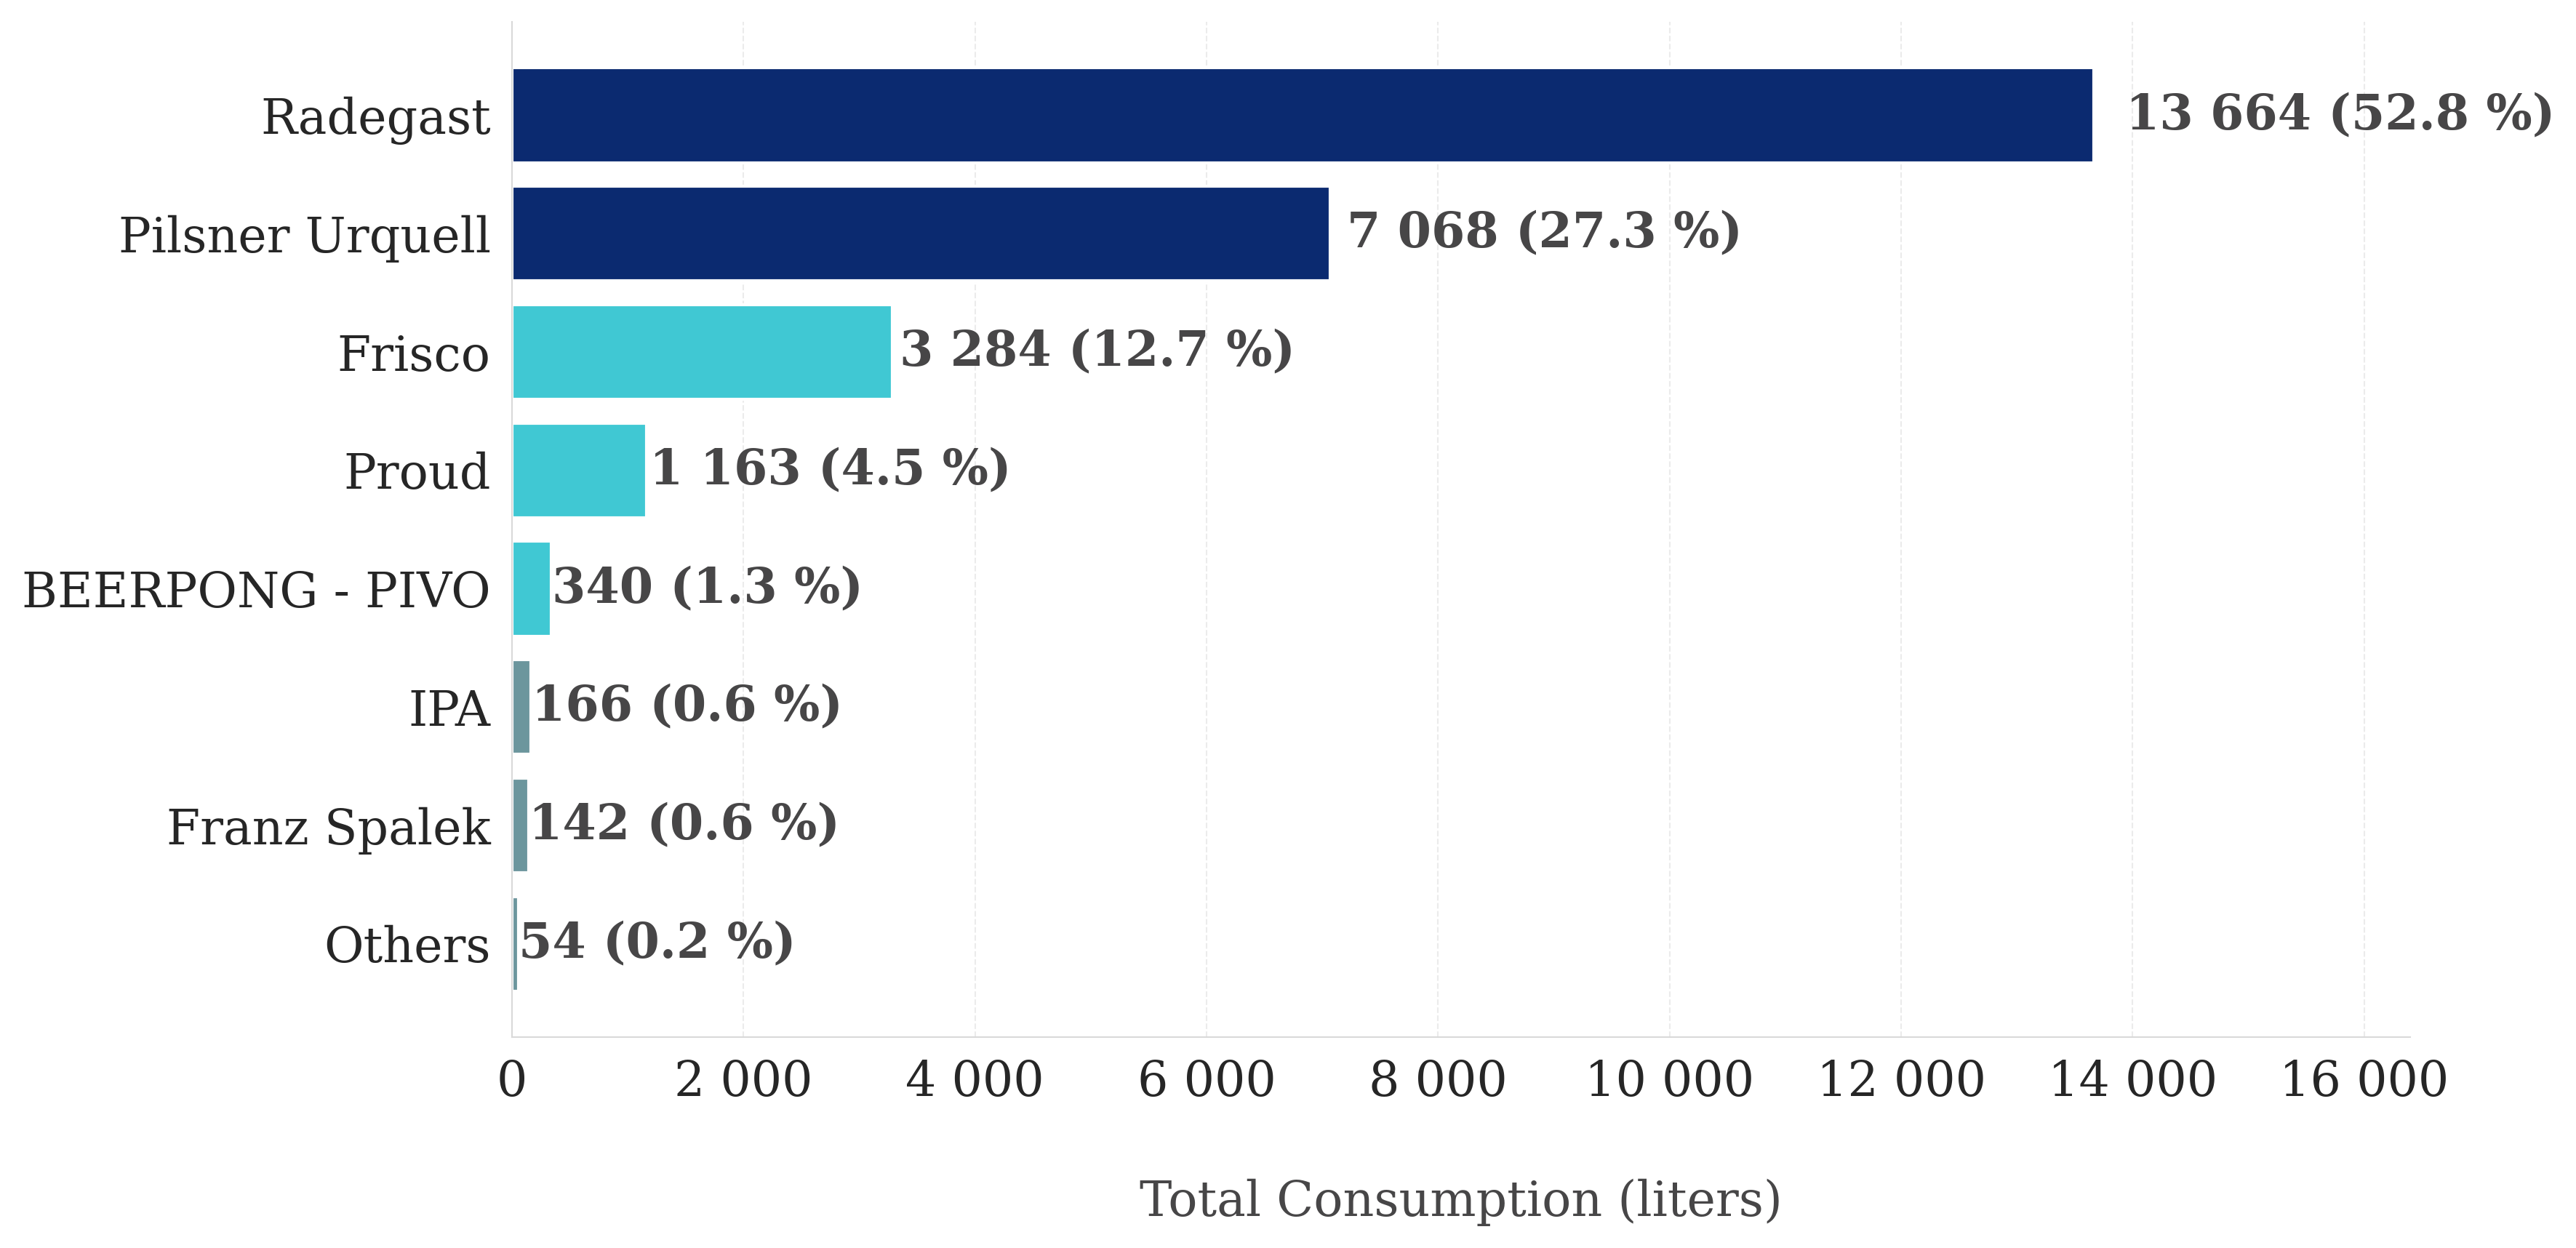
\includegraphics[width=0.99\textwidth]{\ResultsDir/rq15-top-beer-brands}
	\caption{Most Consumed Beer Brands}
	\label{fig:beverage-top-beer}
	\source
\end{figure}

This distribution indicates that the most consumed beer brand was \textbf{Radegast}, with a total consumption of~\bfmtnum{10366}~liters and~\bfmtnum{27329} units sold.

The second was \textbf{Pilsner Urquell}, which had half the consumption of \textbf{Radegast}, followed by the \textbf{Frisco} and \textbf{Proud} brands.
A complete list of all ten brands from the festival is shown in the~\autoref{tab:beverage-top-beer}~below.

\begin{table}[htbp]
	\centering
	\small
	\begin{tabularx}{\textwidth}{
		|>{\columncolor{unicorn_blue!5}\centering\arraybackslash}p{1cm}
		|>{\columncolor{unicorn_blue!5}\raggedright\arraybackslash}X
		|>{\columncolor{unicorn_blue!5}\raggedleft\arraybackslash}p{4cm}
		|>{\columncolor{unicorn_blue!5}\raggedleft\arraybackslash}p{2.5cm}|}
		\hline
		\rowcolor{unicorn_blue}
		\textbf{}
		& \textbf{\color{white}Beer brand}
		& \textbf{\color{white}Total consumption}
		& \textbf{\color{white}Units sold}
		\\\hline\hline
% rows
		\csvreader[
			head to column names,
			late after line={\\\hline},
		]{\ResultsDir/rq15-top-beer-brands.csv}{
			subcategory=\colbrand,
			total_consumption_ml=\colconsumption,
			transaction_count=\coltrxcount,
			total_sold=\colunits
		}{
			\the\numexpr\thecsvinputline-1
			& \colbrand
			& \num[group-separator={,}]{\colconsumption}~l
			& \num[group-separator={,}]{\colunits}
		}
		\hline
		\noalign{\vspace{1mm}}
		\hline
		\rowcolor{unicorn_blue!20}
		\textbf{}
		& \textbf{Total}
		& {\bfmtnum{19793}}~l
		& {\bfmtnum{53990}}
		\\\hline
	\end{tabularx}
	\caption{Most Consumed Beer Brands}
	\label{tab:beverage-top-beer}
\end{table}

The data demonstrate a strong preference for Radegast beer among festival attendees.
The price may have influenced this, as the Radegast was generally slightly less expensive than, for instance, the Pilsner Urquell.

\begin{keytakeaways}
	\begin{itemize}
		\item The most consumed beer brand was \textbf{Radegast} with a total of~\bfmtnum{10366}~liters consumed.
		\item The second most consumed beer brand was the \textbf{Pilsner Urquell} with half the consumption of the Radegast.
	\end{itemize}
\end{keytakeaways}

%%% Beverage / Popular Brands Analysis / Non-alcoholic Brands Analysis
%%% --------------------------------------------------------------

\subsubsection{Non-alcoholic Brands Analysis}
\label{subsubsec:analysis-beverage-popular-non-alcoholic}

This next section is bound to the non-alcoholic beverages, which were the second most consumed category.

\begin{rqbox}
	\textit{\researchq{beverage-top-non-alcoholic}}
\end{rqbox}

Aggregated similarly as in the previous analysis, the results in the~\autoref{tab:beverage-top-non-alcoholic}~below show the distribution of the most consumed non-alcoholic brands during the event.

\begin{table}[htbp]
	\centering
	\small
	\begin{tabularx}{\textwidth}{
		|>{\columncolor{unicorn_blue!5}\centering\arraybackslash}p{1cm}
		|>{\columncolor{unicorn_blue!5}\raggedright\arraybackslash}X
		|>{\columncolor{unicorn_blue!5}\raggedleft\arraybackslash}p{4cm}
		|>{\columncolor{unicorn_blue!5}\raggedleft\arraybackslash}p{2.5cm}|}
		\hline
		\rowcolor{unicorn_blue}
		\textbf{}
		& \textbf{\color{white}Non-alcoholic brand}
		& \textbf{\color{white}Total consumption}
		& \textbf{\color{white}Units sold}
		\\\hline\hline
% rows
		\csvreader[
			head to column names,
			late after line={\\\hline},
		]{\ResultsDir/rq17-top-non-alco-brands.csv}{
			subcategory=\colbrand,
			total_consumption_ml=\colconsumption,
			transaction_count=\coltrxcount,
			total_sold=\colunits
		}{
			\the\numexpr\thecsvinputline-1
			& \colbrand
			& \num[group-separator={,}]{\colconsumption}~l
			& \num[group-separator={,}]{\colunits}
		}
		\hline
		\noalign{\vspace{1mm}}
		\hline
		\rowcolor{unicorn_blue!20}
		\textbf{}
		& \textbf{Total}
		& {\bfmtnum{6971}}~l
		& {\bfmtnum{20487}}
		\\\hline
	\end{tabularx}
	\caption{Most Consumed Non-alcoholic Brands}
	\label{tab:beverage-top-non-alcoholic}
\end{table}

The results indicate a close rivalry between the \textbf{Birell} and \textbf{ZON Lemonade} brands, with Birell emerging as the most consumed non-alcoholic beverage at the event.
A total of~\bfmtnum{6971}~liters drank and~\bfmtnum{20487}~units sold established it as the most popular non-alcoholic beverage, commanding a~\bfmtnump[2]{31.35}\%~share of the total consumption.

\begin{keytakeaways}
	\begin{itemize}
		\item The most consumed non-alcoholic brand was \textbf{Birell} with a total of~\bfmtnum{2186}~liters consumed.
		\item The second most consumed non-alcoholic brand was the \textbf{ZON Lemonade}.
	\end{itemize}
\end{keytakeaways}

%%% Beverage / Popular Brands Analysis / Alcoholic Brands Analysis
%%% --------------------------------------------------------------

\subsubsection{Alcoholic Brands Analysis}
\label{subsubsec:analysis-beverage-popular-alcoholic}

The last part of this section focuses on other alcoholic beverages, such as spirits, shots, cocktails, and other alcoholic beverages.

\begin{rqbox}
	\textit{\researchq{beverage-top-alcoholic}}
\end{rqbox}

This analysis consisted of a total of 23 different brands consisting mostly of spirits and shots.
Results presented in this section may be more biased than the previous ones, as the brand determination was more difficult due to the lack of consistent labeling.
Moreover, previously it was necessary to classify the products with the volume information, which is not so straightforward for shots and spirits.

The results in the~\autoref{tab:beverage-top-alcoholic}~indicate that the most consumed alcoholic brand was the \textbf{Beefeater} with a total of~\bfmtnum{966}~liters consumed and~\bfmtnum{4628}~units sold.
However, the second most consumed brand was \textbf{Absolut Vodka} with only \bfmtnum{335}~liters consumed, but with a much higher units sold count of~\bfmtnum{9177}.

\begin{table}[htbp]
	\centering
	\small
	\begin{tabularx}{\textwidth}{
		|>{\columncolor{unicorn_blue!5}\centering\arraybackslash}p{1cm}
		|>{\columncolor{unicorn_blue!5}\raggedright\arraybackslash}X
		|>{\columncolor{unicorn_blue!5}\raggedleft\arraybackslash}p{4cm}
		|>{\columncolor{unicorn_blue!5}\raggedleft\arraybackslash}p{2.5cm}|}
		\hline
		\rowcolor{unicorn_blue}
		\textbf{}
		& \textbf{\color{white}Alcoholic brand}
		& \textbf{\color{white}Total consumption}
		& \textbf{\color{white}Units sold}
		\\\hline\hline
% rows
		\csvreader[
			head to column names,
			late after line={\\\hline},
		]{\ResultsDir/rq16-top-alco-brands.csv}{
			subcategory=\colbrand,
			total_consumption_ml=\colconsumption,
			transaction_count=\coltrxcount,
			total_sold=\colunits
		}{
			\the\numexpr\thecsvinputline-1
			& \colbrand
			& \num[group-separator={,}]{\colconsumption}~l
			& \num[group-separator={,}]{\colunits}
		}
		\hline
		\noalign{\vspace{1mm}}
		\hline
		\rowcolor{unicorn_blue!20}
		\textbf{}
		& \textbf{Total}
		& {\bfmtnum{1980}}~l
		& {\bfmtnum{26964}}
		\\\hline
	\end{tabularx}
	\caption{Most Consumed Alcoholic Brands}
	\label{tab:beverage-top-alcoholic}
\end{table}

\begin{keytakeaways}
	\begin{itemize}
		\item The most consumed alcoholic brand was the \textbf{Beefeater} with a total of~\bfmtnum{966}~liters consumed.
		\item The second most consumed alcoholic brand was the \textbf{Absolut Vodka} with a total of~\bfmtnum{335}~liters consumed.
	\end{itemize}
\end{keytakeaways}

%%% Beverage / Summary
%%% --------------------------------------------------------------

\subsection{Summary}
\label{subsec:analysis-beverage-consumption-summary}

Insights into beverage consumption, covered in this section, should provide a better understanding of the overall preferences and total consumptions during the festival.
As this data was not previously available, it was a valuable addition to the analysis and will play a significant role when presenting the results to the festival organizers.

The results showed the total consumption of all beverages, the insightful view on returnable cups usage, and the most consumed beverage brands in the most popular categories.

With the data available, there are still many more questions that could be answered, particularly in combination with customer data.
However, clear bounds were set for this analysis to answer the most important questions asked by the festival organizers.

The next section will focus on the customer analysis to get a better understanding of the festival visitors and their behavior.

%%% Section: Customer Analysis
%%% --------------------------------------------------------------


\section{Customer Analysis}
\label{sec:analysis-customers}

This section will focus on customer analysis, which should provide interesting insights into festival attendees' behavior and segmentation.

Because the organizers lacked deeper insights into festival attendees, this analysis should contribute significantly to a better understanding of the event.

The analysis addresses the remaining fourteen research questions, which have been reorganized into four logical groups to improve the narrative flow:
\begin{enumerate}
	\item \fullref{subsec:analysis-customer-event-attendance-timeline}
	\begin{itemize}
		\small
		\item \textit{\researchq{customers-total-attendance}}
		\item \textit{\researchq{customers-new-visitors}}
		\item \textit{\researchq{customers-visitor-time}}
		\item \textit{\researchq{customers-top-up-peaks}}
	\end{itemize}
	\item \fullref{subsec:analysis-customer-segmentation-engagement}
	\begin{itemize}
		\small
		\item \textit{\researchq{customers-top-up-online}}
		\item \textit{\researchq{customers-mobile-app}}
		\item \textit{\researchq{customers-distribution-types}}
		\item \textit{\researchq{customers-visitors-types-difference}}
	\end{itemize}
	\item \fullref{subsec:analysis-customer-payment-behavior}
	\begin{itemize}
		\small
		\item \textit{\researchq{customers-bank-cards}}
		\item \textit{\researchq{customers-card-schemes}}
		\item \textit{\researchq{customers-top-up-more-than-once}}
		\item \textit{\researchq{customers-visitors-difference}}
	\end{itemize}
	\item and~\fullref{subsec:analysis-customer-purchase-pattern}
	\begin{itemize}
		\small
		\item \textit{\researchq{customers-drink-preferences}}
		\item \textit{\researchq{customers-common-combinations}}
	\end{itemize}
\end{enumerate}

%%% Customer / Event Attendance and Timeline Analysis
%%% --------------------------------------------------------------

\subsection{Event Attendance and Timeline Analysis}
\label{subsec:analysis-customer-event-attendance-timeline}

This section should provide information about attendees' initial behavior, total attendance throughout the festival, and subsequent top-up behavior.

%%% Customer / Event Attendance and Timeline Analysis / Total Attendance and Daily Activity
%%% --------------------------------------------------------------

\subsubsection{Total Attendance and Daily Activity}
\label{subsubsec:analysis-total-attendance}

\begin{rqbox}
	\textit{\researchq{customers-total-attendance}}
\end{rqbox}

The analysis shows that the festival attracted a total of~\bfmtnum{10009}~unique customers over the three-day duration.
However, the daily attendance figures show interesting patterns in how these customers were distributed throughout the festival days.

Looking at the daily active customers:
\begin{itemize}
	\item Day 1 (Thursday):~\bfmtnum{6214}~active customers
	\item Day 2 (Friday):~\bfmtnum{5832}~active customers
	\item Day 3 (Saturday):~\bfmtnum{8066}~active customers
\end{itemize}

These numbers indicate that many customers attended multiple days of the festival, as the sum of daily attendees (\bfmtnum{20112}) is significantly higher than the unique customer count.
This was expected, as the festival was designed to attract visitors for multiple days.

The attendance peaked on the final day of the festival, with Day 2 showing slightly lower attendance than the opening day.
The significant increase in attendance on Day 3 suggests that the festival successfully attracted weekend visitors.

\begin{keytakeaways}
	\begin{itemize}
		\item Total unique customers over the three days:~\bfmtnum{10009}.
		\item The highest attendance was on Day 3 (Saturday) with~\bfmtnum{8066}~active customers.
		\item The festival maintained consistent attendance on weekdays (Days 1–2).
		\item Significant increase in attendance (38\% higher than Day 2) for the weekend (Day 3).
	\end{itemize}
\end{keytakeaways}

%%% Customer / Event Attendance and Timeline Analysis / Visitor Arrival Patterns
%%% --------------------------------------------------------------

\subsubsection{Visitor Arrival Patterns}
\label{subsubsec:analysis-visitor-patterns}

\begin{rqbox}
	\textit{\researchq{customers-new-visitors}}
\end{rqbox}

The analysis of visitor arrival patterns reveals distinct peak periods across the three festival days, with significant variations in the rate of new visitor registrations throughout each day.

\begin{figure}[H]
	\centering
	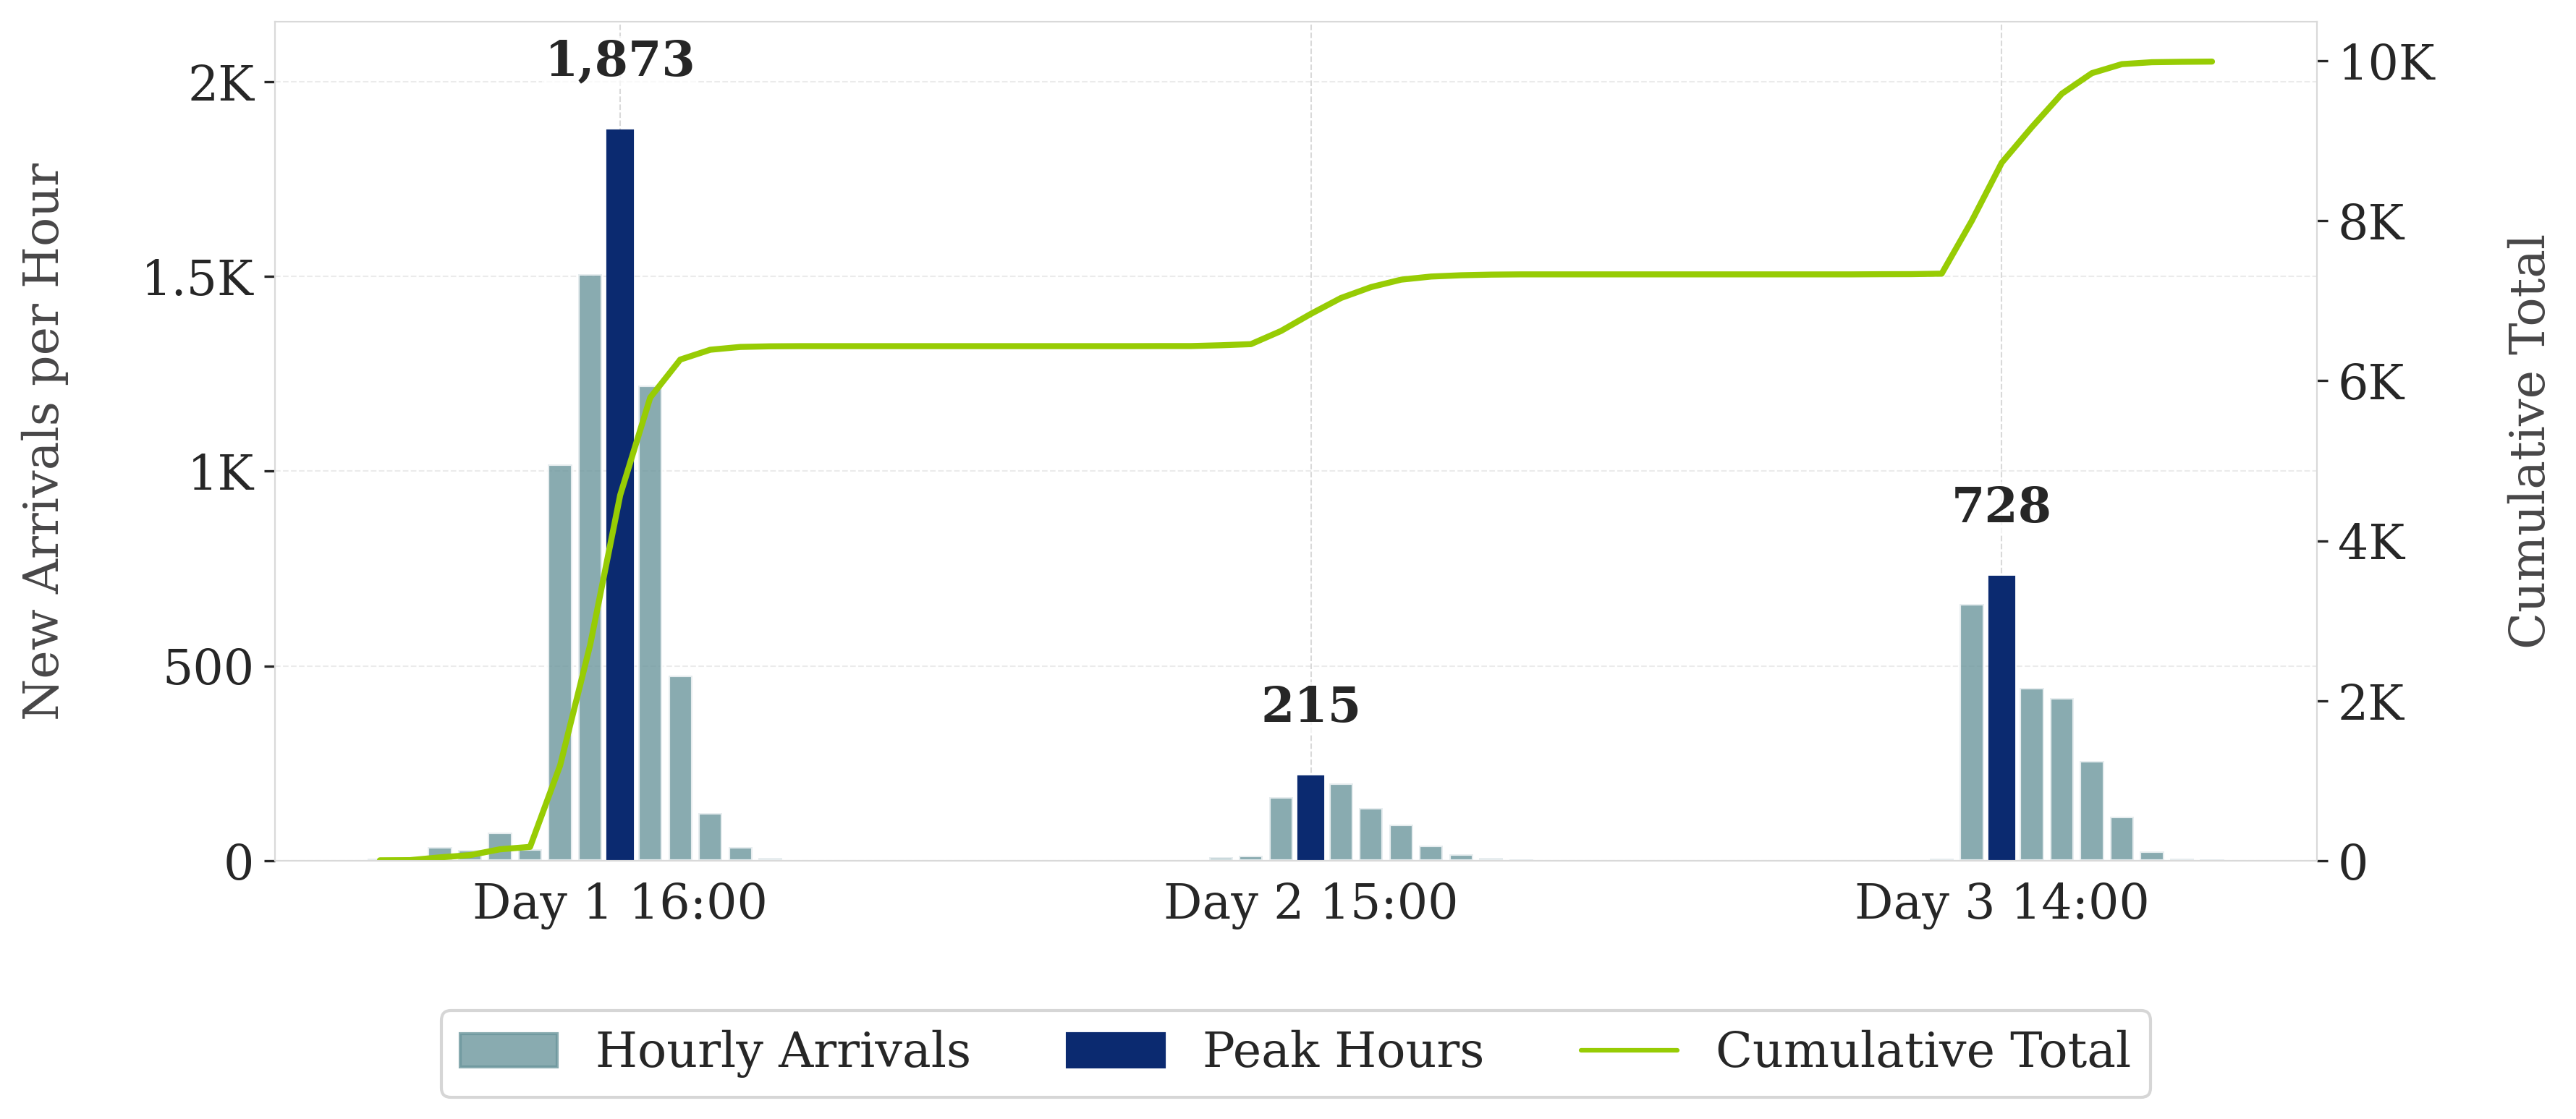
\includegraphics[width=0.99\textwidth]{\ResultsDir/rq21-arrival-patterns}
	\caption{Visitor Arrival Patterns}
	\label{fig:visitor-arrival-patterns}
%	TODO add and use \source elsewhere also!
	\source
\end{figure}

The data reveals three distinct patterns across the festival days:

\begin{itemize}
	\item \textbf{Day 1 (Thursday)}: A rapid peak of approximately~\bfmtnum{1873}~new visitors was observed during the 16:00 hour, which was the time of the highest registration activity.
	\subitem The day showed a clear pattern of increasing registrations from 14:00 to 16:00, followed by a gradual decline.
	\item \textbf{Day 2 (Friday)}: A modest peak of~\bfmtnum{215}~visitors at 15:00, but significantly lower new registrations than on Day 1.
	\subitem This decrease in the number of new registrations was expected, as a significant number of visitors had already completed the registration process on Day 1.
	\item \textbf{Day 3 (Saturday)}: The weekend attendees' influx was clear in the resurgence of new registrations, which reached a peak of~\bfmtnum{728}~new visitors at 14:00.
\end{itemize}

The data indicates that the majority of visitor registrations occurred during the afternoon hours (14:00–17:00) on all days.
Minimal new registrations were consistently observed during the early morning hours (before 10:00) and late evening hours (after 20:00).

\begin{keytakeaways}
	\begin{itemize}
		\item Highest single-hour registration peak:~\bfmtnum{1873}~visitors (Day 1, 16:00).
		\item The registration window that was most effective was from 14:00 to 17:00 on all days.
		\item Day 1 accounted for approximately~\bfmtnump[2]{64.39}\%~of total registrations.
		\item Weekend (Day 3) saw renewed registration activity with peak of~\bfmtnum{728}~new visitors.
	\end{itemize}
\end{keytakeaways}

%%% Customer / Event Attendance and Timeline Analysis / Top-Up Peaks
%%% --------------------------------------------------------------

\subsubsection{Time to First Transaction}
\label{subsubsec:analysis-first-transaction}

\begin{rqbox}
	\textit{\researchq{customers-visitor-time}}
\end{rqbox}

The analysis reveals significant variations in how quickly different types of visitors made their first transaction after arrival.
Overall, the average time to the first transaction was~\bfmtnum{79.55}~minutes.
However, this number alone is misleading, as evidenced by the much lower median of~\bfmtnum{7}~minutes and mode of~\bfmtnum{3}~minutes.

\begin{figure}[H]
	\centering
	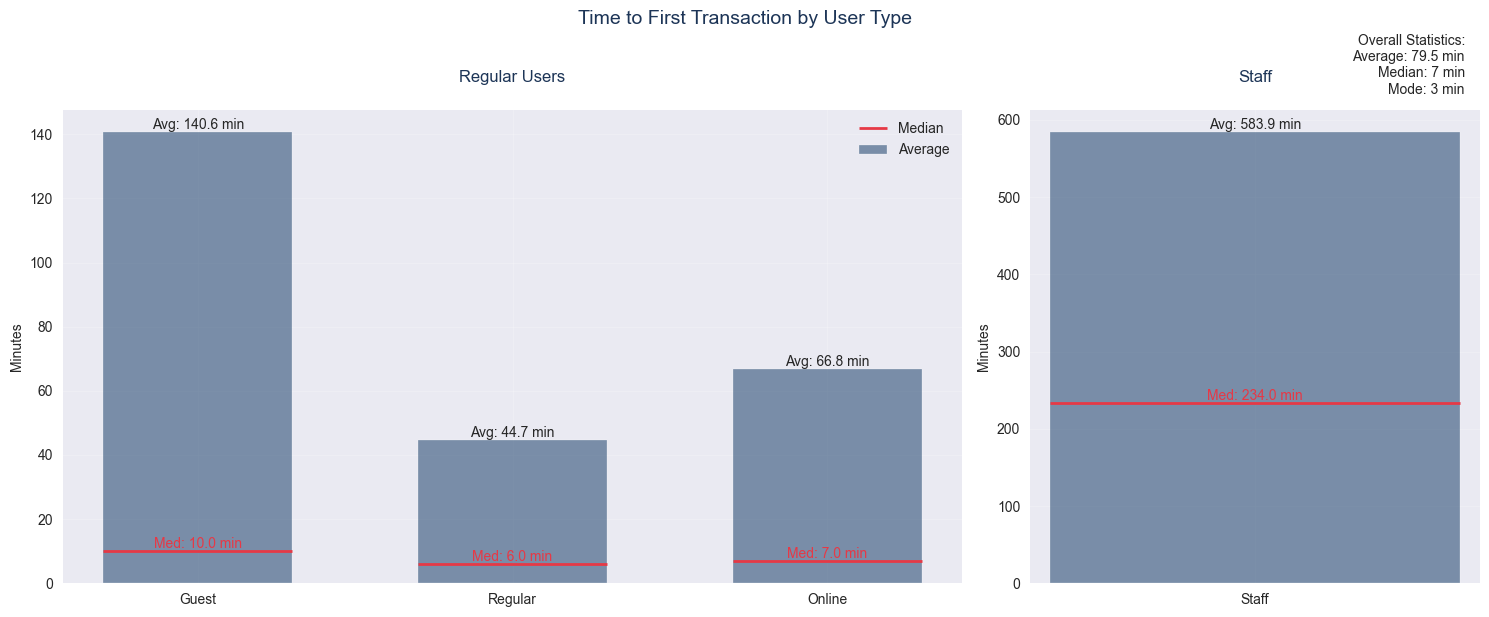
\includegraphics[width=0.99\textwidth]{\ResultsDir/rq22-time-to-first-transaction}
	\caption{Time from Arrival to First Transaction Analysis}
	\label{fig:time-to-first-transaction}
	\source
\end{figure}

Breaking down the analysis by visitor type\footnote{Visitor or rather, chip types are described in the~\fullref{tab:chip-types} table.}, reveals distinct patterns:

\begin{itemize}
	\item \textbf{Regular}: Quickest to transact, with an average of \bfmtnum{44.68} minutes and a median of only \bfmtnum{6} minutes
	\item \textbf{Online}: Similar efficiency with an average of \bfmtnum{66.85} minutes and a median of \bfmtnum{7} minutes
	\item \textbf{Guests}: Took longer, averaging \bfmtnum{140.59} minutes with a median of \bfmtnum{10} minutes
	\item \textbf{Staff}: Showed significantly different behavior, with an average of \bfmtnum{583.92} minutes and a median of \bfmtnum{234} minutes
\end{itemize}

\begin{table}[H]
	\centering
	\small
	\begin{tabularx}{\textwidth}{
		|>{\columncolor{unicorn_blue!5}\centering\arraybackslash}l
		|>{\columncolor{unicorn_blue!5}\raggedleft\arraybackslash}X
		|>{\columncolor{unicorn_blue!5}\raggedleft\arraybackslash}X
		|>{\columncolor{unicorn_blue!5}\raggedleft\arraybackslash}X
		|>{\columncolor{unicorn_blue!5}\raggedleft\arraybackslash}X|
	}
		\hline
		\rowcolor{unicorn_blue}
		\textbf{\color{white}Visitor Type}
		& \textbf{\color{white}Average}
		& \textbf{\color{white}Mode}
		& \textbf{\color{white}Median}
		& \textbf{\color{white}Max}
		\\
		\hline
		\colorindicator{chart1}Guest
		& \bfmtnum{140.59}~min
		& \bfmtnum{0}~min
		& \bfmtnum{10}~min
		& \bfmtnum{3176}~min
		\\
		\colorindicator{chart2}Regular
		& \bfmtnum{44.68}~min
		& \bfmtnum{0}~min
		& \bfmtnum{6}~min
		& \bfmtnum{2852}~min
		\\
		\colorindicator{chart3}Online
		& \bfmtnum{66.85}~min
		& \bfmtnum{3}~min
		& \bfmtnum{7}~min
		& \bfmtnum{3199}~min
		\\
		\colorindicator{chart4}Staff
		& \bfmtnum{583.92}~min
		& \bfmtnum{7}~min
		& \bfmtnum{234}~min
		& \bfmtnum{3492}~min
		\\
		\hline
		\rowcolor{unicorn_blue!20}
		\textbf{Overall}
		& \bfmtnum{79.55}~min
		& \bfmtnum{3}~min
		& \bfmtnum{7}~min
		& \bfmtnum{3492}~min
		\\
		\hline
	\end{tabularx}
	\caption{Time from Arrival to First Transaction}
	\label{tab:time-to-first-transaction}
	\source
\end{table}

The significant difference between average and median times across all categories suggests a right-skewed distribution, implying that while most visitors completed their first transaction quickly, others took much longer.
This was especially true for regular attendees, who would sometimes arrive early to check in and then return later to make their first purchase.

Staff members who were not there primarily to consume, on the other hand, exhibited a different behavior pattern, with their first transaction occurring later.
This was most likely due to their responsibilities at the event, which may have prevented them from making purchases during working hours.

\begin{keytakeaways}
	\begin{itemize}
		\item Most visitors (as indicated by the median) made their first transaction within~\bfmtnum{7}~minutes of arrival.
		\item Regular visitors were the most efficient, typically transacting within~\bfmtnum{6}~minutes.
		\item Staff members showed distinctly different behavior, likely due to their different role at the event.
		\item The large gap between mean and median times suggests some visitors waited significantly longer than others before their first transaction.
	\end{itemize}
\end{keytakeaways}

\subsection{Customer Segmentation and Digital Engagement}
\label{subsec:analysis-customer-segmentation-engagement}
\todo{Distribution and characteristics of customer types, Analysis of online vs on-site customer behavior, Digital service adoption (mobile app, online top-ups), Comparative analysis of spending patterns across segments, Impact of digital channels on customer behavior}
% TODO
\begin{rqbox}
	\textit{\researchq{customers-top-up-online}}
\end{rqbox}
% TODO
\begin{rqbox}
	\textit{\researchq{customers-mobile-app}}
\end{rqbox}
% TODO
\begin{rqbox}
	\textit{\researchq{customers-distribution-types}}
\end{rqbox}
% TODO
\begin{rqbox}
	\textit{\researchq{customers-visitors-types-difference}}
\end{rqbox}

\subsection{Payment Behavior Analysis}
\label{subsec:analysis-customer-payment-behavior}
\todo{Analysis of payment methods and card schemes, Credit top-up frequency patterns, Duration-based analysis of customer spending, Credit management across different visitor types, Insights for future payment system optimization}
% TODO
\begin{rqbox}
	\textit{\researchq{customers-bank-cards}}
\end{rqbox}
% TODO
\begin{rqbox}
	\textit{\researchq{customers-card-schemes}}
\end{rqbox}
% TODO
\begin{rqbox}
	\textit{\researchq{customers-top-up-more-than-once}}
\end{rqbox}
% TODO
\begin{rqbox}
	\textit{\researchq{customers-visitors-difference}}
\end{rqbox}

\subsection{Purchase Pattern Analysis}
\label{subsec:analysis-customer-purchase-pattern}
\todo{Temporal analysis of drink preferences, Product combination analysis, Purchase behavior insights, Implications for inventory and service optimization}
% TODO
\begin{rqbox}
	\textit{\researchq{customers-drink-preferences}}
\end{rqbox}
% TODO
\begin{rqbox}
	\textit{\researchq{customers-common-combinations}}
\end{rqbox}